% !TeX root = ./main.tex
% !TEX program = pdflatex
% !TEX encoding = UTF-8 Unicode
% !TEX options = --shell-escape -synctex=1 -interaction=nonstopmode -file-line-error "%DOC%"
\documentclass[final]{kuee_en}
\usepackage[titletoc]{appendix}

% citation
\usepackage[final,breaklinks=true]{hyperref}
\renewcommand*{\sectionautorefname}{Section}
\renewcommand*{\chapterautorefname}{Chapter}
% \usepackage{cleveref}

% put all the figures end
\usepackage[nomarkers,
    % disable,
    ]{endfloat}
\renewcommand{\efloatseparator}{\mbox{}}

\usepackage{amsfonts}
\usepackage{amssymb}
\usepackage{xcolor,graphicx}
\usepackage{subcaption}
\usepackage{sectsty} % change section style
\sectionfont{\noindent\textsc} % indent setting
% \usepackage{paralist}
% \usepackage{booktabs}
\usepackage[utf8]{inputenc}
\usepackage[T1]{fontenc}
\usepackage{tgbonum}
\usepackage{fancyhdr}

% svg insert
\usepackage[inkscape=on]{svg}
\svgpath{{imgs/svg/}}
\usepackage[off]{svg-extract}
\svgsetup{%
	extractpath=./imgs/svg-extract/,
	inkscapepath=./imgs/svg-inkscape, 
	clean=true,
	convertformat={png},
	convertdpi={png=600},%
	convertdpi=300}

% using modern biblatex
\usepackage[sorting=none,
    % backend=biber,
    bibencoding=utf8,
    bibstyle=nature,
    doi=false,isbn=false,url=false,eprint=false]{biblatex}
\bibliography{library}
\bibliography{bibsupple}

%%%%%%%%%% Start TeXmacs macros
\newcommand{\mathd}{\mathrm{d}}
\newcommand{\tmname}[1]{\textsc{#1}}
\newcommand{\tmop}[1]{\ensuremath{\operatorname{#1}}}
\newcommand{\tmtextit}[1]{{\itshape{#1}}}
\newcommand{\nosymbol}{}
\newcommand{\tmmathmd}[1]{\ensuremath{#1}}
%%%%%%%%%% End TeXmacs macros

\newcommand\mycaption[2]{\caption[#1]{\textbf{#1}. #2}}
\newcommand{\dint}{D_\mathrm{int}}

\etitle{Broadband frequency entangled photon generation using silicon nitride ring cavities}
% \title{\cjk{窒化シリコンリング共振器を用いた\\広帯域周波数もつれ光子生成}}
\title{Broadband frequency entangled photon generation using silicon nitride ring cavities}
\eauthor{Zhenghao Yin} 
\author{\cjk{殷 政浩}}
\supervisor{\cjk{竹内 繁樹 教授}}
\school{\cjk{京都大学大学院工学研究科}}
\depart{\cjk{電子工学専攻}}
\date{\cjk{令和2年2月1日}}

\begin{document}
\maketitle

\begin{abstract}
    \lipsum[1]
\end{abstract}

\tableofcontents
% \clearpage


% !TeX root = ../main.tex
\chapter{Introduction}

\section{Background}

Quantum mechanics has not only boosted up the modern science and technology in different disciplines, but also established the cornerstone for future quantum information processing technology. 
Furthermore, differing from the past applications of quantum mechanics which only involves the quantization nature, the frontier quantum information processing 
including but not limited to quantum computation, quantum communication and quantum metrology, 
exploits the deep-level physics of quantum mechanics, such as quantum superposition and quantum entanglement.
Therefore, the fundamental quanta of light---photon---featuring attractive advantages like long coherent time and multiple degrees of freedom (DoF), is a suitable candidate among the research quantum computation and quantum communication. 

Furthermore, entanglement between photon pairs which originates from the nonlocality of quantum mechanics, can be easily realized using nonlinear bulk crystals. 
While in the term of DoF, much of research up to now focuses on the polarization and path entanglement approaches and very little attention has been paid to frequency entanglement, whose basis is continuous and infinite in hilbert space. 
Moreover, the previous research shows that frequency entangled photon pairs can be exploited not only in wavelength division multiplexing quantum key distribution \cite{Wengerowsky2018} but also promising to transfer quantum information in future quantum networks \cite{Tchebotareva2019}. 
An example of quantum computation is cluster state encoded by frequency \cites{Reimer2019}.
Therefore, frequency entangled photon plays a powerful and general role for optical quantum information processing.

Nevertheless, large scale realization of frequency entanglement requires hundreds of free-space optical components, especially the nonlinear crystals, which challenges robust manipulation of generated quantum states.
Besides, in recent applications of quantum metrology, quantum optical coherent tomography (QOCT), the broadband frequency entanglement \cite{Okano2015} is also urgent.

To improve both scalability and robustness, chip-scale full-optical routine has been developed for optical quantum information processing \cites{ Vahala2008, OBrien2009}.  
A conventional material candidate is silicon on insulator (SOI), since it is CMOS compatible and supplied by silicon wafer manufacturers. Much of research up to date reported not only frequency \cite{Kues2017b} but also path and time-bin encoded quantum state in this platform \cites{Paesani2018,Zhang2018a}. Other materials like lithium niobate and aluminum nitride are also developed and show various advantages, but requires special fabrication technology.

\section{Objective}

However, suffering from two photon absorption and stimulated Raman scattering \cite{Engin2012}, silicon is no able to generate high-intensity and broadband frequency conversion. 
Since that, silicon nitride, which is transparent from visible to near infrared range, can be used to achieve ultra-broadband frequency conversion. 
A simple comparison of these two material is shown in \autoref{tab:si-vs-sin}.
Recently, single photon pair generation from visible to telecom band is reported\cite{Lu2016}. 

\begin{table}[]
	\mycaption{Comparison of several material properties between silicon and silicon nitride}{The data of silicon is cited from Reference \cite{Sinclair2019} and silicon nitride refers to \cite{Ang2018}.}
	\label{tab:si-vs-sin}
	\begin{tabular}{ccc}
							& silicon nitride 			& silicon		 			\\ \hline
		refractive index $n$ at 1550 nm
							& 2.0						& 3.4						\\ \hline
		transparent band 	& visible to NIR			& NIR					    \\ \hline
		two photon absorption $ \beta_\mathrm{TPA} $ (cm/GW)                 
							& - 						& 0.75 			 			\\ \hline
		Kerr nonlinearity $ n_2 $ (\si{\square\meter\per\watt})             
							& \num{6.94d-19} 			& \num{5d-18} 				\\ \hline
	\end{tabular}
\end{table}

In the silicon nitride waveguide, third-order optical nonlinearity is dominant and leads spontaneous four wave mixing in sub-micron scale. 
To enhance the nonlinear interaction, the all-pass ring resonator is used where the light is coupled inside from a bus waveguide. Once continuous wave laser launched at the ring resonant mode, the cavity made of nonlinear material is strongly driven and leads frequency broadening nature intracavity. Thus, other resonant modes are excited and then photon are generated spontaneously. Indeed, this progress is governed by phase matching condition in nonlinear optics.
In our research, by carefully optimizing the device geometry, broadband phase matching condition can be realized. 
Finally, all the photon pair generation events are detected by single photon detectors and verified by the coincident counting.
%In this dissertation, the terms 'broadband photon pair' is used to describe that pairs are generated in different frequency pairs simultaneously and but entangled only in the single mode pair. 

\newpage

\section{Outline}
The following chapters are sequentially divided in different topics.

% !TeX root = ../main.tex

\chapter{Principal theory}

The way how light travels in a chip-scale is remarkably different the way in free-space. In the sub-micron scale, the electromagnetic wave can only propagate in a fewer cycles due to the constraint of material boundaries. However, since atoms and molecules are much smaller, the refractive index is not changed, as well as the reflection, interference and diffraction. 

Based on these facts, in order to perform quantum optics experiments \textit{at the bottom}, first, we shall confine the light propagation in a specific waveguide. On the other hand, thanks to modern laser technology, nonlinear optics is involved and give birth to optical frequency conversion. To enhance these nonlinear optical phenomena, we adopt the cavity structure and achieve sizable control.

In this chapter, we briefly introduce the guided wave theory and then move the cavity structure, ring resonators. Next, the nonlinear optics, in particular third-order nonlinear processes, is discussed in the following section. Although the quantum nature of photon pair generation distinct from the classical theory, all the physics mentioned above are necessary to analyse our essential research object, the silicon nitride ring resonators.


\section{Guided-wave optics}\label{sec:guide}

In an ideal optical waveguide, the core layer and the cladding layer are usually composed of two different materials, where the refractive index is larger in the core. As an analogue of optical fibers, only in the higher index region can the light propagate, and meanwhile dissipate in a wavelength scale in the lower index region.

Usually, we assume the core and the cladding layer are made of nonmagnetic (magnetic permeability $\mu = \mu_0$) and dielectric material (conductivity $\sigma = 0$). Furthermore, we neglect the nonlinear response of the polarization of electric field ($\vb{P} \simeq \varepsilon_0 \chi \vb{E}$).

Since the waveguide in numerous research objects, is deposited or sputtered using chemical or physical methods, the uneven density in the waveguide layer can not be negligible. Hence, the propagation equation derived from Maxwell's equation is
\begin{equation}\label{eq:aniso}
  (\nabla_{\perp}^2 + k^2 n^2 - \beta^2) \vb{E} = - (\nabla_{\perp} + i
  \beta \hat{\vb{z}}) (\vb{E_{\perp}} \nosymbol \cdot \nabla_{\perp} \ln
  n^2)
\end{equation}
where $\perp$ denotes the transverse component, $\nabla_{\perp}^2 = \nabla_x^2 + \nabla_y^2$. And $k, n, \beta$ are the wave vector in vacuum, refractive index and propagation constant, respectively. While, with the negligible film anisotripy, \autoref{eq:aniso} can be approximated into
\begin{equation}\label{eq:helm}
  (\nabla_{\perp}^2 + k^2 n^2 - \beta^2) \vb{E} = 0
\end{equation}
This is the normal \textit{Helmholtz equation}, indicating the relation between propagation constant $\beta$ and material refractive index, i.e. \textit{chromatic dispersion}.

Next, the boundary conditions determining the solution to Eqn. \ref{eq:helm}, arise from the Maxwell's equations as well.
\begin{eqnarray*}%\label{eq:bcon}
  \vb{\hat{n}} \cdot (\vb{E_a - E_b}) & = & 0 \\
  \vb{\hat{n}} \times (\vb{\vb{H_a} - H_{\vb{b}}}) & = & 0
\end{eqnarray*}
which is the continuity condition of both electric and magnetic field at all dielectric material interfaces. Here, $\vb{\hat{n}}$ is the normal direction at the material boundary and the subscript $a, b$ denote different regions.

\subsection{Waveguide modes}
In the case of channel waveguides, the index discontinuity from both vertical and horizontal sides can be decomposed into two sets of independent and complete conditions, i.e. the horizontal boundary condition and vertical boundary condition, with the discontinuity on the waveguide corners neglected. In other words, approximately the equation has two independent partiuclar solutions, which is the mathematical origin of \textit{ transverse electric} (TE) modes and \textit{transverse magnetic} (TM) modes.

\begin{figure}
\centering
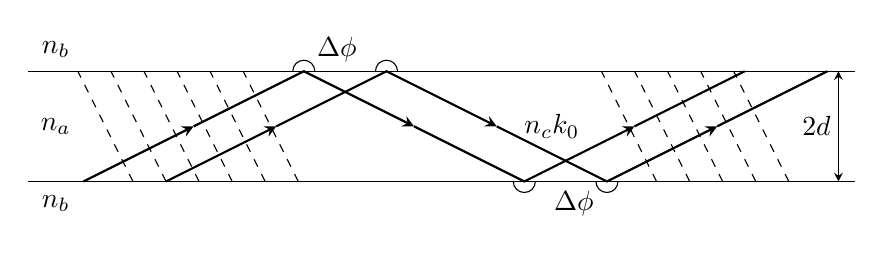
\begin{tikzpicture}[scale=0.7,>=stealth]
\draw (-9,0) -- (6,0) (-9,2) -- (6,2);
% \draw [->] (-9,1) -- (6,1);
\foreach \x in {0,1.5}{
  \draw [thick, ->] (-8+\x,0) -- (-6+\x,1);
  \draw [thick,->] (-6+\x,1) -- (-4+\x,2) -- (-2+\x,1);
  \draw [thick,->] (-2+\x,1) -- (0+\x,0) -- (2+\x,1);
  \draw [thick,-] (2+\x,1) -- (4+\x,2);
}
\foreach \x in {-1,0,1,2,3,4}
	\draw [dashed] (-6.5+0.6*\x,0) -- (-7.5+0.6*\x,2);
\foreach \x in {0,1,2,3,4}
	\draw [dashed] (2.4+0.6*\x,0) -- (1.4+0.6*\x,2);

% \draw [<->] (-9,1.5) --(-9,0.7) -- (-7.4,0.7);
% \draw [->] (-9,0.7) -- (-7.4,1.5);

% \node at (-8.6,1.4) {$\tiny{k_i}$};
% \node at (-8.2,0.4) {$\tiny{\beta}$};
\node at (0.5,1) {$n_c k_0$};

\draw [<->] (5.7,0) -- (5.7,2);
\node at (5.3,1) {$2d$};
\node at (-8.5,1) {$n_a$};
\node at (-8.5,2.4) {$n_b$};
\node at (-8.5,-0.4) {$n_b$};
\node at (-3.4,2.4) {$\Delta\phi$};
\node at (0.9,-0.4) {$\Delta\phi$};

\draw (-3.8,2) arc [start angle=0, end angle=180, radius=0.2];
\draw (-3.8+1.5,2) arc [start angle=0, end angle=180, radius=0.2];

\draw (-3.8+3.6,0) arc [start angle=180, end angle=360, radius=0.2];
\draw (-3.8+5.1,0) arc [start angle=180, end angle=360, radius=0.2];
\end{tikzpicture}
\mycaption{Planar waveguide}{The upper and bottom layer are cladding and the middle is core layer. $\Delta \phi$ represents the Goos-H\"{a}nchen shift at the boundary.}
\label{fig:planar}
\end{figure}

Hence, we can study the eigenequantion by selecting only one set of boundary condition, as used in the \textit{the effective index method}. For example, in a planar waveguide shown in \autoref{fig:planar} ,$\dv*[2]{}{y}=0$\footnote{Since the planar waveguide is infinite at the $y$-direction , thus the solution is identical in arbitrary $xz$-plane, which means no gradient along $x$-axis.},
the TE mode features $E_x=0$ and consider only $y$-component, 
\begin{equation}
    \dv[2]{E_y}{x} + (k^2 n^2 - \beta^2)E_y =0
\end{equation}
and $E_y$ is continous at $x=\pm d/2$, where $d$ is the thickness of core layer.

For the region $|x|>d/2$, the light evanesces at $x$-direction at rate $\kappa$ and in contrast, in the region of core layer, the light performs like stationary wave, denoting with $k_x$. By substituting these conditions, phase continuity is achieved between two interface

\begin{equation}\label{eq:te-eq}
    2k_x d = m\pi + 2\arctan(\kappa/k_x)
\end{equation}
where $m$ is the index of stationary wave. The second term can be treated as the Goos-H\"{a}nchen phase shift. Overall, the waveguide modes characterize that the phase shall maintain itself with an $m\pi$ shift along with the shift at the boundaries.

In the case of TM modes, the eigen equation is 
\begin{equation}\label{eq:tm-eq}
    2k_x d = m\pi + 2\arctan(\delta\kappa/k_x)
\end{equation}
where $\delta=n_a/n_b$ is the index ratio and only differs from \autoref{eq:te-eq} with this parameter. conclusively, the less is $\delta$ parameter, the propagation constant of TE and TM modes are closer.

\subsection{Dispersion relation}
Based on \autoref{eq:te-eq} and \autoref{eq:tm-eq}, $k_x$ can be solved and then utilized to calculate propagation constant $\beta$, since $n_a^2k^2 = k_{\perp}^2 + \beta^2$. In the case of channel waveguides, the TE and TM solutions are both necessary. Therefore, propagation constants $\beta$ can be expressed as the product of free space wave vector $k$ and the \textit{ effective index} $n_{\mathrm{eff}}$
\begin{equation}\label{eq:disp_bk}
    \beta = n_{\mathrm{eff}}k = n_{\mathrm{eff}}(\lambda) \frac{2\pi}{\lambda} = n_{\mathrm{eff}}(\omega) \frac{\omega}{c}
\end{equation}
along with the differential form
\begin{align}\label{eq:ng-def}
    \dv{\beta}{k} &= n_{\mathrm{eff}} + k \dv{n_{\mathrm{eff}}}{k} = n_{\mathrm{eff}} - \lambda\dv{n_{\mathrm{eff}}}{\lambda} \equiv n_g \\
    \dv{\omega}{\beta} &= c \dv{k}{\beta} = \frac{c}{n_g} \equiv v_g  
\end{align}
which defines the group index $n_g$ and group velocity $v_g$.

This formula linking $\beta - k$ or $\beta - \omega$ is named as dispersion relation, which gives the physics that light with different color propagates at different \textit{speed}. Furthermore, \autoref{eq:te-eq} and \autoref{eq:tm-eq} also indicate that the dispersion relation intrinsically depends on waveguide geometry.

\section{Ring resonators}

The ring resonators comprise of a bus waveguide and a ring waveguide, are usually demonstrated as optical filters or modulators at a wide range of platforms. The working principle of ring resonator can be derived completely \cite{Bogaerts2012} as an analogue to Fabry-P\'{e}rot etalon, based on the coupling mode theory. 

\begin{figure}
    \centering
	\includesvg{mrr_illus}
	\mycaption{An all-pass type ring resonator}{The transmitted spectrum is filtered periodically by the ring waveguide, in the case satisfying resonance condition.}
    \label{fig:mrr-illus}
\end{figure}

In the model illustrated in \autoref{fig:mrr-illus}, the self-coupling coefficient $\tau$ and the cross-coupling coefficient $\kappa$ can be evaluated analytically or using numerical simulation. Assuming the coupling only occur at the very close area, $\tau,\kappa$ are the power splitting ratios of the coupler and satify $\tau^2 + \kappa^2 =1 $ if the coupling section is lossless. $a$ is the single-pass amplitude transmission, including both propagation loss in the ring and loss in the couplers.

\begin{figure}
    \centering
    \includesvg{mrr_cp}
    \mycaption{The transmission spectrum of a ring resonator}{}
    \label{fig:mrr_spec}
\end{figure}

The transmission rate of a all-pass type ring cavity takes the form of
\begin{equation}\label{eq:trans_phi}
    T = \frac{I_\mathrm{pass}}{I_\mathrm{input}} = \frac{a^2 - 2a\tau \cos \phi + \tau^2}{1 - 2ar \cos \phi + a^2 \tau^2}
\end{equation}
where $\phi=\beta L$ is the phase shift in a single round trip. 

\subsection{Coupling condition}

By plotting the function in \autoref{fig:mrr_spec}, we can see, the extinction ratio of absorption peak is defined by the self-coupling coefficient $\tau$ and the single-pass amplitude transmission $a$ due to device geometric differences, like the gap between the bus waveguide and the ring cavity. Namely, $a$ and $\tau$ both determine the coupling condition, which can be categorized in three cases
\begin{itemize}
    \item \textbf{weak coupling} $a>\tau$. The loss inside the ring is larger than the power coupled from bus waveguides.
    \item \textbf{critical coupling} $a=\tau$. The loss and self-coupling are in balance. The optical power restored in the resonator achieve the minimum.
    \item \textbf{over coupling or strong coupling} $a<\tau$. The coupling is too strong for the light to dissipate in a single round trip.
\end{itemize}

Previous work \cite{Yusuke2017} proposed a method to evaluate the coupling condition above using the experimentally measured device transmission. Considering the loss in the coupler, bent segment of ring and higher mode perturbance, usually the critical coupling varies from modes and the cross section of waveguides \cite{Pfeiffer2017}.

\subsection{Spectrum characteristics}
Meanwhile, the minimum of transmission rate $T$ can be achieved periodically as $\phi=2 m \pi$, which defines the resonance of ring resonators. Therefore, the resonance condition is derived as
\begin{equation}\label{eq:res-con}
    \beta L =2 m \pi
\end{equation}
where $m$ is the mode index. Specifically, the propagation constant $\beta$, shall be an integral times of a quasi wave vector $2\pi/L$. With this condition, the free spectral range (FSR) of wavelength and frequency are obtained
\begin{align}
    \Delta \lambda_\mathrm{FSR} &\approx \frac{\lambda_\mathrm{res}^2}{n_g L} \label{eq:fsr-wl} \\
    \Delta \omega_\mathrm{FSR} &\approx \frac{2\pi c}{n_g L} \label{eq:fsr-w}
\end{align}

In both wavelength and frequency domain, FSR determines the spacing of neighbouring resonant peak. This is a significant factor when the ring resonators are designed.

Furthermore, from \autoref{eq:trans_phi}, the full width at half maximum (FWHM) of the resonance spectrum is derived as $\delta\lambda$
\begin{equation}\label{eq:fwhm_phi}
    \delta\phi = \frac{2(1- a \tau)}{\sqrt{\tau a}}
    % \lambda_{\mathrm{res}}^2
\end{equation}
\begin{figure}
    \centering
    \includesvg{mrr_fsr_illus}
    \mycaption{Illustration of wavelength transmission spectrum of ring resonators}{FSR, free spectral range, the distance between neighbouring resonant wavelength. FWHM, full width at half maximum.}
    \label{fig:my_label}
\end{figure}

Likely, since the phase $\phi$ is related with the wave vector $k$ in \autoref{eq:ng-def}. Substituting $\delta \phi = L n_g \delta k$, the half width of wavelength is
\begin{equation}
    \delta \lambda = \dv{\lambda}{k}\delta k = \frac{\lambda_\mathrm{res}^2}{2\pi L n_g} \frac{2(1- a \tau)}{\sqrt{\tau a}} \label{eq:fwhm_wl}
\end{equation}
the same, at the frequency domain
\begin{equation}
    \delta \omega = \dv{\omega}{k}\delta k = \frac{c}{ L n_g} \frac{2(1- a \tau)}{\sqrt{\tau a}} \label{eq:fwhm_w}
\end{equation}

Note in \autoref{eq:fsr-wl} \autoref{eq:fsr-w} \autoref{eq:fwhm_wl} and \autoref{eq:fwhm_w}, the group index $n_g$ is explicit instead of the effective index $n_\mathrm{eff}$ because both free spectral range and full width depend on the differential form, \autoref{eq:ng-def}.

And the finesse $F$ of the resonator is defined 
\begin{equation}
    F \equiv \frac{2\pi}{\delta\phi} = \frac{\pi\sqrt{\tau a}}{2(1- a \tau)}
\end{equation}

Finally, we define the quality factor, a measure of the sharpness of the resonance relative to its central frequency.

\begin{equation}\label{eq:q-def}
    Q = \frac{\lambda_\mathrm{res}}{\delta \lambda} =  \frac{\pi L n_g \sqrt{\tau a}} {\lambda_\mathrm{res} (1- a \tau)}
\end{equation}

Usually, the \textit{Q}-factor can be decomposed into two parts by formula $Q^{-1}=Q_{i}^{-1} + Q_{l}^{-1}$. And $Q_{i}, Q_{l}$ are intrinsic \textit{Q}-factor and loaded \textit{Q}-factor, referring to the loss inside the ring waveguide and at the coupler, respectively. The physical meaning of the finesse and \textit{Q}-factor relates to the number of round-trips before being lost to internal loss and the bus waveguides when the power is depleted to $1/e$ of its initial value.

\section{Thrid-order nonlinear optics}

Although the nonlinear effect is ignored during the derivation of waveguide modes in \autoref{sec:guide}, 
for numerous materials, the nonlinear response of electric field is significant even at mW level, which is easy to occur with assistance of modern lasers. The origin of nonlinear optic phenomena is similar to the movement of the object in a potential field, such as the ball-spring model. 

In the nonlinear material, the atoms or molecules are driven by the external electric field, due to the around chemical bonds or molecular orientation, the displacement of atoms or molecules perform nonlinear dependence on the strength of field. In real-world materials, interaction coming arising from various frequency leads to the addition or subtraction of these frequency components. This explains the frequency conversion nature in nonlinear optics.

% these phenomena are widely used in quantum optics, such as spontaneous parametric down conversion. And
It is worth mentioning that not only in the bulk crystals, but also in the sub-micron scale \cite{Leuthold2010}, the nonlinear response is still efficient, even over a single-layer two-dimensional material.

% In this section, we prefer to introduce both second-order and third-order optical nonlinearity. 
Here, a brief theoretical derivation is elucidated and in the following part, degenerate four wave mixing is emphasized. In an isotropic nonlinear medium, assuming only instantaneous dielectric response, the relation between the polarization and the electric field is expressed by a power series in the electric field
\begin{equation}\label{eq:nlp}
    \vb{P}(t) = \varepsilon_0 \large (\chi^{(1)}\vb{E}(t) + \chi^{(2)}\vb{E}^2(t) + \chi^{(3)}\vb{E}^3(t))
    = \varepsilon_0 \chi^{(1)}\vb{E}(t) + \vb{P}_\mathrm{NL}(t)
\end{equation}

Note in \autoref{eq:nlp}, the nonlinear susceptibilities $\chi^{(2)}$ and $\chi^{(3)}$ are second-rank and third-rank tensors, corresponding to the tensor product with $\vb{E}^2$ and $\vb{E}^3$. The higher order response is neglected and sequentially, only $\chi^{(2)}$ processes and $\chi^{(3)}$ processes are to be introduced.

\bigskip
\noindent\textbf{$\chi^{(2)}$ processes} 

In centrosymmetric crystals such as silicon, the second-order susceptibility term is absent. However, in other materials like lithium niobate (\ce{LiNbO3}) and aluminium nitride (AlN), the second-order nonlinearity are essential to realize electro-optic modulation and second harmonic generation.

\bigskip
\noindent\textbf{$\chi^{(3)}$ processes} 

Silicon and silicon nitride are both cubic crystal. Due to the third-order dependence, another factor equivalent to the optical intensity is involved, the $\chi^{(3)}$ process is also named as intensity-dependent effect or Kerr effect.

Consider three frequency components of $\vb{E}^3$, using the complex expression of electric field
\begin{equation}
    \vb{E}(\vb{r}, t) = \sum_{k=1}^3 \vb{E}_{\omega_k}(\vb{r}, t) =  \frac{1}{2} \sum_{k=1}^3 \qty ( \vb{E}_{\omega_k}(\vb{r})e^{i\omega_k t} + c.c.)
\end{equation}
\begin{figure}
    \includesvg{energy_diagram}
    \mycaption{Illustration of possible energy diagram in typical third-order nonlinear processes}{}
    \label{fig:energy-level}
\end{figure}
Substituting into third-order term in \autoref{eq:nlp} and arranging with the same propagation direction, the third-order polarization is 

\begin{align}
  \vb{P}^{(3)}(t) 
  & = \frac{3}{4} \varepsilon_0 \chi^{(3)} \left[| \vb{E}_{\omega_1} |^2 \vb{E}_{\omega_1} + \cdots\right] & \mathrm{SPM} \\
  & + \frac{6}{4} \varepsilon_0 \chi^{(3)} \left[(| \vb{E}_{\omega_2} |^2 + |\vb{E}_{\omega_3} |^2) \vb{E}_{\omega_1} + \cdots \right] & \mathrm{XPM} \\
  & + \frac{1}{4} \varepsilon_0 \chi^{(3)} \left[(\vb{E}_{\omega_1}^3 e^{i \omega_1 t} + c.c.) + \cdots\right] & \mathrm{THG} \\
%   \tag{\stepcounter{equation}\theequation}
  & + \frac{3}{4} \varepsilon_0 \chi^{(3)} \left[ \frac{1}{2} (\vb{E}_{\omega_1}^2 \vb{E}_{\omega_2} e^{i (2 \omega_1 + \omega_2) t} + c.c.) + \cdots \right] & \mathrm{FWM} \label{eq:fwm1} \\ 
  & + \frac{3}{4} \varepsilon_0 \chi^{(3)} \left[ \frac{1}{2} (\vb{E}_{\omega_1}^2 \vb{E}^{\ast}_{\omega_2} e^{i (2 \omega_1 - \omega_2) t} + c.c.) + \cdots \right] & \mathrm{FWM} \label{eq:fwm2} \\ 
  & + \frac{6}{4} \varepsilon_0 \chi^{(3)} \left[ \frac{1}{2} (\vb{E}_{\omega_1} \vb{E}_{\omega_2} \vb{E}_{\omega_3} e^{i (\omega_1 + \omega_2 + \omega_3) t} + c.c.) + \cdots \right] & \mathrm{FWM}  \label{eq:fwm3} \\
  & + \frac{6}{4} \varepsilon_0 \chi^{(3)} \left[ \frac{1}{2} (\vb{E}_{\omega_1} \vb{E}_{\omega_2} \vb{E}^{\ast}_{\omega_3} e^{i (\omega_1 + \omega_2 - \omega_3) t} + c.c.) + \cdots \right] & \mathrm{FWM} \label{eq:fwm4}
\end{align}

In above equations, $\cdots$ stands for all possible permutation terms contributed by frequencies $\omega_1, \omega_2, \omega_3$. The abbreviation on the right side represent for 

\bigskip
\noindent\textbf{SPM, self-phase modulation}

SPM adds an intensity-dependent term except the linear polarization, leading to a broadening of the pulse spectrum.

Note the $\chi^{(3)}$ is complex, thus the imaginary part may contribute to another intensity-dependent absorption mechanics, which is usually depicted in the \textit{two-photon absorption} (TPA). The free carriers excited by TPA in further change the temporally both the absorption coefficient and the refractive index of material.
\begin{equation}\label{eq:spm-index}
    n = n_0 + n_2 I + i \frac{\lambda}{4\pi}(\alpha_0 + \alpha_2 I)
\end{equation}
where the $I$ is the intensity, $n_2$ is the Kerr coefficient and $\alpha_0, \alpha_2$ are related with TPA-induced free carrier absorption (FCA) and free carrier index (FCI) change, both interrelated with third-order susceptibility
\begin{align}
    n_2     &= \frac{1}{cn_0^2\varepsilon_0} \frac{3}{4} \Re{\chi^{(3)}} \\
    \alpha_2&= \frac{-\omega}{c^2n_0^2\varepsilon_0} \frac{3}{2} \Im{\chi^{(3)}}
\end{align}
A figure of merit (FOM) is often used to compare the magnitude of Kerr coefficient $n_2$ with the strength of the TPA coefficient $\alpha_2$
\begin{equation}
    \mathrm{FOM} = \frac{1}{\lambda} \frac{n_2}{\alpha_2}
\end{equation}

\bigskip
\noindent\textbf{XPM, cross-phase modulation} 

XPM can be seen the first signal index influenced by a second signal. And the coeffiecient of XPM is twice as strong as the SPM coefficient.

\bigskip
\noindent\textbf{THG, third-harmonic generation} 

Like SHG, THG generated a new frequency with is one-third of input frequency. 

\bigskip
\noindent\textbf{FWM, four wave mixing} 

% \item DFWM, degenerate four wave mixing
% Another factor to mention is that the coefficient in each $\chi^{(3)}$ process arises from the combination of three frequency components. For instance, on the numerator \autoref{eq:def-dfwm} has the factor 3 but \autoref{eq:def-ndfwm} has the factor 6. 
In FWM process, more than three frequencies are involved. Nevertheless, \autoref{eq:fwm1} and \autoref{eq:fwm2} contain two identical wave, sometime calles as degenerate four wave mixing (DFWM). And \autoref{eq:fwm3} and \autoref{eq:fwm4} is a truly four wave process. Similar to the relation between SPM and XPM, the non-degenerate FWM is naturally twice stronger.

Traditionally, following the terminology in laser field, in DFWM, the $\omega_1$ square term \autoref{eq:fwm2} is labeled as pump frequency, and another two frequencies are referred to signal and idler frequency.

\bigskip
Besides, the imaginary part of third-order susceptibility incorporate other four-wave absorption mechanics, such as \textit{stimulated Brillouin scatter} (SBS) and \textit{stimulated Raman scattering} (SRS), which originate from acoustic waves in crystals and vibrating molecules.

Finally, it worth mentioning that in all THG and FWM processes, different from SPM and XPM processes, phase matching condition is required due to the complex exponential factors. In this case, the phase mismatch can change the polarization rapidly and leads to periodical variation in these parametric processes.

% \section{Nonlinear integrated devices}


% !TeX root = ../main.tex

\chapter{Phase match condition for spontaneous four wave mixing in a ring cavity }\label{chap:pmc-sfwm}

According to the previous chapter, in a typical nonlinear optical waveguide or silica fibers, despite the stimulated Raman and Brillouin scattering, the frequency conversion processes involve not only the self-phase modulation of pump light and cross-phase modulation of signal and idler light, but also the phase mismatch in four wave mixing propagation factor. 
%\begin{equation}\label{key}
%	\Delta \phi = \Delta_M
%\end{equation}
In this case, it is necessary to study the coupled nonlinear equations involving signal, idler and pump intensity \cite{AGRAWAL2013397}. 

Whereas in ring resonators, whose mode linewidth (pm) is much narrower than self-phase modulation frequency broadening, 
the frequency broadening in single mode is negligible. 
Thus the phase mismatch among cavity modes becomes the critical factor of the band of four wave mixing.

This chapter first describes the major origin of phase mismatch, chromatic dispersion, and goes on to the design philosophy used in device fabrication. Besides, several topics concerning the band of phase matching are also included.

\section{Chromatic dispersion}

In a typical FWM process, both energy conservation and momentum conservation are required 
\begin{align}
  \beta_i + \beta_s & = 2 \beta_p \label{eq:beta-cons} \\
  \omega_i + \omega_s & = 2 \omega_p \label{eq:omega-cons}
\end{align}
where the subscripts $s~i~p$ stand for signal, idler and pump light.

Meanwhile, the resonance condition \autoref{eq:res-con} leads to $\beta = m \frac{2 \pi}{L}$. Thus, \autoref{eq:beta-cons} is equivalent to 
\begin{equation}\label{eq:mu-cons}
  m_i + m_s = 2 m_p 
\end{equation} 
  
We can see that \tmtextit{the momentum conservation agrees with mode number
conservation.} That is to say, as pump light sets into resonant wavelengths, by choosing the equidistant modes relative to the pump mode, the momentum conservation can be naturally satisfied. This is the most important difference from non-resonant devices.

Therefore, we can estimate the phase mismatch only in the frequency domain. Expand the resonant frequency into Taylor seires at $\omega_0$ to the propagation constant $\beta$
\begin{eqnarray}\label{eq:omega-taylor}
  \omega_{\mu} & = & \omega_0 
  + \sum_{j=1}\dv[j]{\omega}{\beta} (\beta_{\mu}-\beta_0) \frac{{(\beta-\beta_0)}^j}{j!} \\
  & = & \omega_0 
  + \sum_{j=1}\dv[j]{\omega}{\beta} \qty(\frac{2 \pi}{L})^j \frac{\mu^j}{j!} \nonumber \\
  & = & \omega_0 + D_1 \mu + \frac{D_2}{2!} \mu^2 + \frac{D_3}{3!} \mu^3 + \cdots \nonumber
\end{eqnarray}
where $D_j \equiv  (\frac{2 \pi}{L})^j\dv*[j]{\omega}{\beta}$ are \textit{j}-order mode number dispersion parameter, whose dimension are all $\mathrm{T}^{-1}$ and $\mu \in \mathbb{Z}$ is the relative mode number. 

It is easy to know that $D_1 / 2 \pi = v_g / L$ is the free spectral range in the frequency and indicates that the dispersion property is related with the difference of resonant frequencies.   

Next, we introduce the integrated dispersion $\dint$ \cite{Brasch2014a} to analyze the phase mismatch
\begin{align}\label{eq:def-dint}
    D_\mathrm{int}(\mu) &\equiv \omega_{\mu} - (\omega_0 + D_1 \mu)  \\
    &= \frac{D_2}{2!} \mu^2 + \frac{D_3}{3!} \mu^3 + \cdots \nonumber
\end{align}

In particular, $\dint$ is the residual dispersion higher than second order. Approximately, if $D_3 \mu \ll D_2$, the second-order dispersion will dominate the integrated dispersion both at signal and idler mode.

Indeed, the mode number dispersion parameter is linked with the dispersion coefficients in frequency and wavelength domain, giving such a chain rule
\begin{equation}\label{eq:disp-chain}
    D_2 = - \frac{L}{2\pi} {D_1^3}{\beta_2} = \frac{L}{2\pi}  \frac{\lambda^2}{2\pi c} {D_1^3} D_{\lambda}
\end{equation}
where $\beta_2=\dv*[2]{\beta}{\omega}$ is group velocity dispersion (GVD) and $D_{\lambda}= - (\lambda/c)\dv*[2]{n}{\lambda}$ is the dispersion parameter.

In this method, we can analyze the phase mismatch in FWM quantitatively
\begin{align}\label{eq:freq-mismatch}
	\Delta \omega &\equiv \omega_s + \omega_i - 2 \omega_p \\
%	&=  D_{\mathrm{int},s} + D_{\mathrm{int},i} \\
	&= \dint(\mu) + \dint(-\mu) \nonumber \\
	&= 2\qty(\frac{D_2 \mu^2}{2!} + \frac{D_4 \mu^4}{4!} + \frac{D_6 \mu^6}{6!} +\cdots)  \nonumber
\end{align}

From the above derivation, the frequency mismatch $ \Delta\omega $ only adds to the even terms of Taylor series in \autoref{eq:omega-taylor}.
To conclude, a rough presupposition to increase the efficient phase matched band is achieving zero and flat dispersion around pump wavelengths.

\section{Dispersion compensation}\label{sec:disp-comp}
Previously mentioned  in \autoref{sec:guide}, the dispersion behaviour in integrated devices is not only the intrinsic material property, but also depends on the waveguide dimension. 

In other words, the phase mismatch occurs as a result of material dispersion $D_M$ and waveguide dispersion $ D_W $, $D_{\lambda}= D_M + D_W$. Here, we adopt the wavelength dispersion parameter since the wavelength domain is measurable.

Usually, the Sellmeier equation is used to fit the refractive index for a particular transparent medium based on the Lorentz-Drude mode. \citeauthor{Luke2015a} reported the below measured refractive index of stoichiometric \ce{Si3N4} film \cite{Luke2015a}
\begin{equation}\label{eq:si3n4-selleimeier}
    n_{\ce{Si3N4}}^2 = 1 + \frac{3.0249 \lambda^2}{\lambda^2-135.3406^2} + \frac{40314 \lambda^2}{\lambda^2 - 1239842^2}
\end{equation}

This Sellmeier equation is valid over the wavelength range 310–5504 \si{\nm}.
The result of \autoref{eq:si3n4-selleimeier} is plotted in \autoref{fig:Luke-si3n4}, along with the material dispersion parameter $D_M$, which is calculated at the precision of \si{\nm} using the second-order finite difference of refractive index. In the telecom C-band, $n$=1.9963 and $D_M$ = -6.57 \dispu, which suggests the material dispersion at this range is considerably small.

\begin{figure}
    \centering
    \includesvg{Luke}
    \mycaption{Refractive index and dispersion parameter measured in reference}{$ \lambda$=1550 \si{\nm}, $n$=1.9963 and $D_M$ = -6.5656 \dispu .}
    \label{fig:Luke-si3n4}
\end{figure}

On the other hand, the numerical simulation is adopted to evaluate the waveguide parameter.
We use commercial software \si{\nm}{Lumerical MODE} to solve for the refractive index of fundamental TE modes.
Shown in \autoref{fig:wg-disp}, the dimension dependence of waveguide dispersion features negative values in the small waveguide size, i.e. behaving as normal dispersion at the second order. Nevertheless, as either the thickness or width of channel waveguide increases,
$D_W$ turns positive. This indicates that to achieve zero dispersion in phase match condition of four wave mixing, the normal material dispersion can be compensated with anomalous waveguide dispersion. 

For example, at 1550 \si{\nm}, in a 1.5-\si{\um}-wide and 0.8-\si{\um}-thick silicon nitride waveguide cladded by silica, where the refractive index is 1.48,
the waveguide dispersion is 45 \dispu. Substituting into the second-order dispersion chain rule in \autoref{eq:disp-chain}, the second-order mode number dispersion parameter $ D_2 $ is about 12 kHz. It is close to zero dispersion for the pump wavelength.

\begin{figure}
	\centering
	\includesvg{fdtd_fine}
	\mycaption{Waveguide dispersion map simulated by Lumerical MODE}{The central wavelength to perform the simulation is 1550 \si{\nm} and the precision is nm. We select the fundamental TE mode as the objective to study the waveguide dispersion. The scattered point in the figure is 1.5-\si{\um}-wide and 0.8-\si{\um}-thick.}
	\label{fig:wg-disp}
\end{figure}

\section[{Dispersion engineering using slot structure}]{Dispersion engineering using \\ slot structure}

The slot waveguide was firstly realized by \citeauthor{Xu2004} experimentally \cite{Xu2004}. The same group, \citeauthor{Almeida2004} then discussed the light enhancement and confinement caused by large discontinuity of the electric field at high-index-contrast interfaces \cite{Almeida2004}. In the recent decade, it is fully studied that such a novel waveguide can be also used to design dispersion-flattened waveguide \cites{Mas2010, Zhang2010, Zhu2012, Nolte2013}, including the both vertical or horizontal and single or multiple slots. It is also reported a micro-ring resonators formed by a slot hybrid waveguide 
exhibits a flat and low anomalous dispersion \cite{Zhang2013}.

In our research, the vertical slot is preferred due to the easy fabrication during the monolithic process. 
%We propose a double-slot silicon nitride to achieve near-zero and flat dispersion.
For example, in a double vertical slot waveguide illustrated in \autoref{fig:slot-illus}, two extra gaps are fully etched and then reburied with low-index medium instead. 
Except the waveguide width $w$ and thickness $t$, two extra parameters are defined, the position factor $ \mathit{pf} $, ratio of slot position to the waveguide width $w$, and the filling factor $ \mathit{ff} $, ratio of slot width to the waveguide width.

\begin{figure}
		\centering	
		\includesvg{slot-illus}
		\mycaption{Illustration of a double vertical slot waveguide}{The cyan region is \ce{Si3N4} waveguide and surrounded by silica.}
		\label{fig:slot-illus}
\end{figure}


\begin{figure}
	\centering
	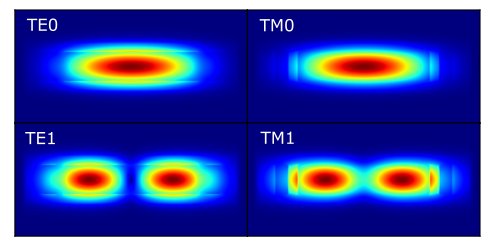
\includegraphics[width=.8\linewidth]{imgs/png/slot_mode}
    \mycaption{Modes of the double vertical slot waveguide}{$w$=2.5, $t$=0.8, $\mathit{ff}$=0.053, $\mathit{pf}$=0.4}
 	\label{fig:slot-mode}
\end{figure}

%\begin{figure}
%	\centering
%	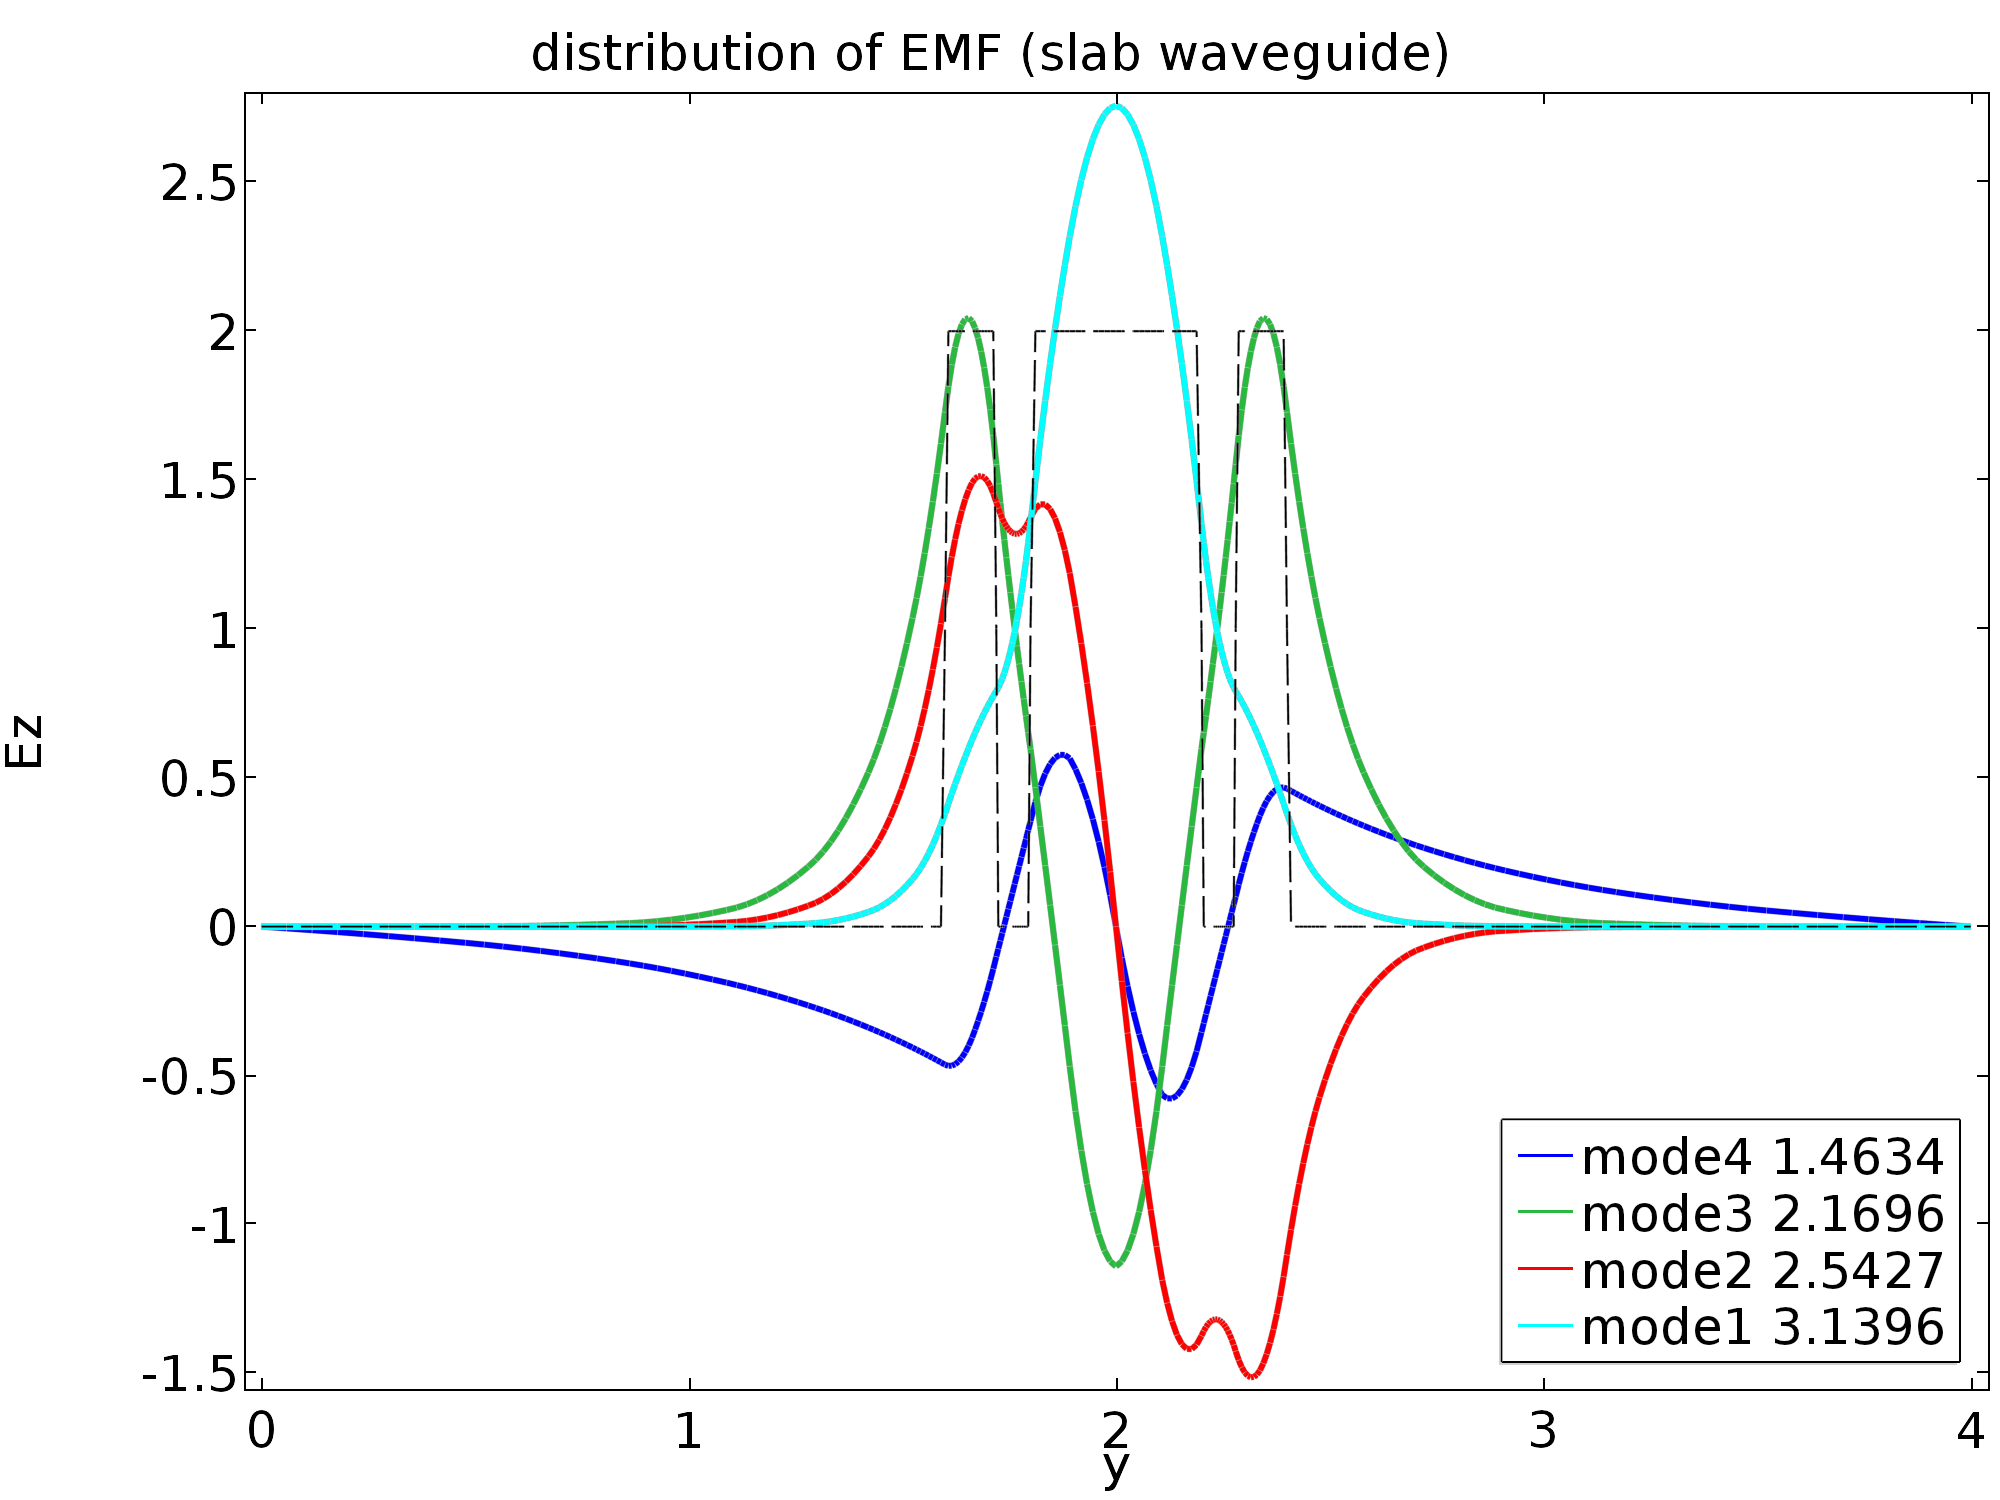
\includegraphics[width=0.7\linewidth]{imgs/png/Ez}
%	\mycaption{Modes of the double vertical slot waveguide}{}
%	\label{fig:slot-mode-Ez}
%\end{figure}

To classify the modes in this slot structure, the same mode solver mention in previous section is performed.
In the result shown in \autoref{fig:slot-mode}, in TM0 and TM1 modes, the light is confined strongly in the slots while the TE0 and TE1 is similar to the normal TE modes, where the discontinuity is obvious on the upper and lower interfaces.

%An interesting finding is that differing from the simple rectangular waveguide, 
%the mode of both quasi-TE and quasi-TM modes can be assumed as the symmetric and anti-symmetric combination of the mode field on both sides. 

%\begin{align}\label{key}
%	\vb{E}_\mathrm{sym} &= \vb{E}_{l} + \vb{E}_{r} \\
%	\vb{E}_\mathrm{asym} &= \vb{E}_{l} - \vb{E}_{r} \nonumber
%\end{align}

%\autoref{fig:slot-mode-Ez} is the \textit{z}-component of the electric field of the four modes. For example, quasi-TE0 mode is even parity while quasi-TE1 mode is odd parity.

Furthermore, by optimizing the position and filling factors, the near-zero and flattened dispersion can be obtained. 


\section{Effects of mode crossing}

In the conclusion of \autoref{sec:disp-comp},
only in the wider or thicker waveguides can the zero dispersion be compensated. However, 
despite the fabrication difficulty arising from thicker films,
the waveguide of larger size also supports high order modes. 

In this case, due to the perturbation of high order modes, the linear mode coupling occurs and influences the resonance spectrum. 
In the study of soliton generation,
it is found that avoided mode crossings induced by linear mode coupling can prevent optical soliton formation when affecting resonator modes close to the pump laser frequency \cites{Herr2014a,Bao2018}. On the other hand, by introducing artificial mode crossing, the anomalous group velocity can also be achieved \cite{Kim2017}. Even though the phenomena mentioned in these works are classical, but in the term of phase matching condition, the physics is similar.

In the following research, the mode crossings found in our devices not only change the spectrum transmission, but also leads to failure of evaluating the dispersion properties.




% !TeX root = ../main.tex

\chapter{Device fabrication of silicon nitride ring resonators}

Different from fabrication of silicon photonic devices based silicon-on-insulator (SOI) wafers, which is CMOS-compatible and widely used in the laboratory and semiconductor industry, to fabricate integrated silicon nitride device, in particular high Q-factor ring resonators realizing four wave mixing, is still challenging.

Collaborating with Yokoyama Lab in Kyushu University, we perform the subtractive fabrication of silicon nitride ring resonators as well as other optical devices. To discover the diversity of fabrication recipes and compare the material properties, we also design the device layout and order the devices using ligentec process and NTT-AT process.

\section{Subtractive fabrication process}

The subtractive process refers to the subtraction of unnecessary parts after the patterning, differing from the lift-off or damascence processes. For optical waevguides, it challenges the etching process to achieve less roughness on the sidewalls. 
% abrication of waveguide is widely perform in a variety of material platforms, including silicon nitride.
The previous work using similar fabrication processes reported silicon nitride ring resonators with \textit{Q}-factor up to \num{5.2d4}. The measured loss of waveguides is 2.9 dB/cm \cite{Cheng2017b}. 

\begin{figure}
	\centering
	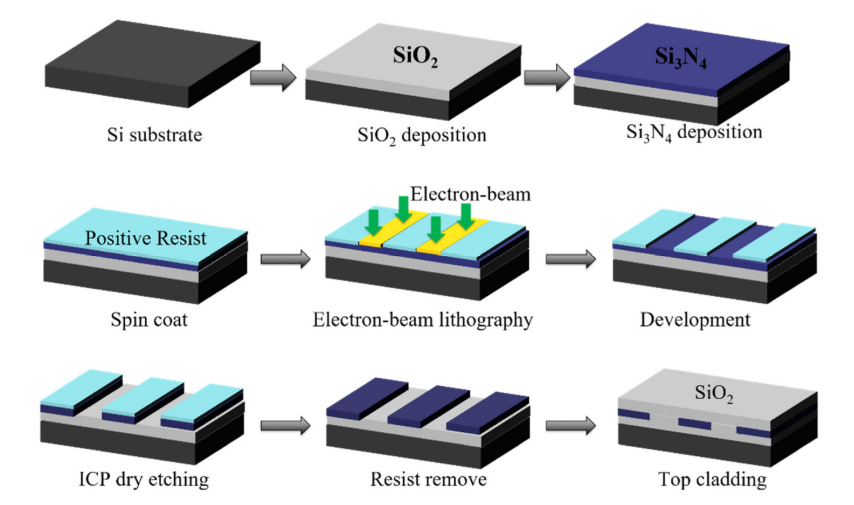
\includegraphics[width=1.0\linewidth]{imgs/png/fab-flow}
	\mycaption{Schematic process flow of the subtractive process}{}
	\label{fig:fab-flow}
\end{figure}

The schematic process flow of the subtractive process is shown in \autoref{fig:fab-flow}. First, the silicon dioxide film is deposited on a 4-inch silicon substrate using the TEOS  (tetraethyl orthosilicate) source.
An alternative method is using a thermal oxidized silicon wafer directly. The target thickness of silicon dioxide layter is greater than 2 \si{\um} to create enough buffer between the silicon nitride film and the silicon substrate. 
Next is silicon nitride film deposition using chemical vapor deposition methods. Following electron beam (EB) lithography patternning, the silicon nitride layer is etched with inductively coupled plasma reactive-ion etching (ICP RIE) technique. After the resist removal, another layer of silica is cladded. Finally, the chip is cut to couple the light from the edge. 

The details of each step will be expanded in the following contents.

%Recently, Si3N4 has been widely utilized in integrated optic devices because of its conspicuous flexibility in the refractive index around 2.0. In our fabrication (Fig. 1), the Si3N4 films with controlled thickness and refractive index were deposited onto the SiO2/Si substrate through LSCVD using the liquid SiN-X source (SAMCO Inc.) with N2 or N2O. The measured refractive index of the deposited Si3N4 film was 1.99, which can be turned to between 1.66 and 1.78 as silicon oxynitride (SiOxNy) by mixing N2O gas. The propagation loss of the films also demonstrated a temperature dependence of the deposition. If the temperature is set too low, the chemical reaction may be uncompleted to form Si3N4. We found that the optimal deposition temperature was 150C to obtain the required low loss properties. The photonic patterns of waveguides, ring resonators, and grating couplers were transferred onto the resist layer on Si3N4 by using the electron beam lithography (EBL) technique. The direct write capability of EBL guarantees the small feature size and high accuracy of the device. After development, the patterned resist was hard-baked at 150C for 5 minutes. This process is effective to improve the dry etching selectivity of the resist and Si3N4, and to help to achieve rectangle waveguide cross-sections. We used a mixed gas of CHF3/O2 for the inductively coupled plasma reactive ion etching (ICP-RIE). After etching to reach the desired depths, we striped the leftover resist using the RIE in which the O2 plasma removes only the resist, but leaves the exposed Si3N4 waveguide untouched. By utilizing CVD, we deposited a top cladding of SiO2 onto the Si3N4 core to form a buried ridge waveguide resonator

\subsection{Film deposition}

Low pressure CVD (LP-CVD) is a traditional method to deposit silicon nitride from the vapor source by the decomposition of chemicals on the surface.  
Stoichiometric silicon nitride can be obtained by controlling and optimizing the ratio of silicon and nitrogen sources. 
The precursor of silicon is usually silane (\ce{SiH4}) or chloride silane gases, such as dichlorosilane (DCS, \ce{SiH2Cl2}). And the ammonia gas (\ce{NH3}) plays the role of nitrogen source. 
\begin{align*}
    \ce{3SiH4(g) + 4NH3(g) &-> Si3N4(s) + 12H2(g)} \\
    \ce{3SiH2Cl2(g) + 4NH3(g) &-> Si3N4(s) + 6HCl(g) + 6H2(g)}
\end{align*}

Considering the toxic gases used in LP-CVD, an alternative approach is to use modern plasma-enhanced CVD (PE-CVD) with liquid source, which has faster growing rate and lower reaction temperature. 

% Although the silicon nitride waveguides deposited by LP-CVD method are mainly reported, it is necessary to figure out the CVD method dependence of film properties, especially the refractive index. 

To compare the CVD method dependence of film properties, especially the refractive index, in our research, three different CVD facilities---LP-CVD, PE-CVD and liquid source CVD (LS-CVD) are exploited with three different recipes to deposit the silicon nitride films.

Compared with commercial silicon nitride on insulator wafers deposited using LP-CVD,
the details of PE-CVD and LS-CVD recipes are listed in \autoref{tab:cvd}. It is apparent from the data that LS-CVD has the fastest rate 23 nm/min, and lowest reaction temperature. In addition, during our experiments, although the flow rate of SN-2 source changes the film growing rate, it does not effect the film stoichiometry and optical properties. 
% This is different from PE-CVD facility used in this research, which can be also used to produce silicon-rich or nitrogen-rich films as controlling the gas ratio.
It is also worth to mention that all the wafer deposited with above three recipes shows no cracks during the fabrication, suggesting low tensile in silicon nitride films.

\begin{table}[]
\centering
\begin{tabular}{cccc}
\hline
              & LP-CVD                            & PE-CVD                                                                                  & LS-CVD                                                                                  \\ \hline
Facility      & -                                 & SAMCO PD-220NL                                                                          & SMACO PD-100ST                                                                          \\ \hline
Source        & DCS:NH3:N2                        & \begin{tabular}[c]{@{}c@{}}\ce{SiH4}:\ce{NH3}:N2\\ =6:5:189 sccm\end{tabular}                     & \begin{tabular}[c]{@{}c@{}}SN-2:\ce{N2}\\ =0.5:30 sccm\end{tabular}                          \\ \hline
Chamber Temp. & 750\si{\celsius}-800\si{\celsius} & \begin{tabular}[c]{@{}c@{}}upper 150\si{\celsius}\\ lower 350\si{\celsius}\end{tabular} & \begin{tabular}[c]{@{}c@{}}upper 150\si{\celsius}\\ lower 180\si{\celsius}\end{tabular} \\ \hline
RF Power      & -                                 & 40 W                                                                                     & 30 W                                                                                     \\ \hline
Deposition Rate          & -                                 & 15 nm/min                                                                               & 23 nm/min                                                                               \\ \hline
\end{tabular}
\mycaption{Recipes of CVD methods used in this research}{In the case of PE-CVD and LS-CVD, upper electrode and lower electrode are set at different temperature. RF power refers to radio frequency power used to excite the precursor gasses.}
\label{tab:cvd}
\end{table}


\subsection{Material properties}

\subsubsection{Fourier-transform infrared spectroscopy}
The vast majority of studies on silicon nitride fabrication processes have found that the hydrogen remaining in the films leads to N-H and Si-H bonds, which causes the optical absorption at S and C band \cites{Ay2004, Agnihotri2000}. To quantitatively clarify these bonds in our film, we perform the Fourier-transform infrared spectroscopy (FTIR) on the top of silicon nitride film.

The measurement is carried out using attenuated total reflection (ATR) method with SHIMADZU ?. In \autoref{fig:ftir}, the absorbance is taken from the difference with background transmittance. It can be seen that except the peak around 800? \si{\per\cm} referring to Si-N stretching mode, two other peaks are located around 2150 and 3350 \si{\per\cm}, corresponding to Si-H and N-H bonds respectively.

Interestingly, there are also two peaks found at 1020 and 1120, indicating Si-O symmetric and asymmetric stretching modes. This result may be explained by the fact that in ATR method, the depth of penetration at this wavelength is less than 1 micron, while the thickness of silicon nitride layers in our experiment is targeted at 800 nm.
% \cite{Shaw2005}


\begin{figure}
    \centering
    \includesvg{ftir}
    \caption{Caption}
    \label{fig:ftir}
\end{figure}

In conclusion, even though the ammonia free recipe is used in LS-CVD method, the film is still hydrogenated while LP-CVD commercial wafers show least N-H absorbance.

\subsubsection{Ellipsometry}


\subsection{Patterning}
The sample used in our experiments are usually in the size of 20 mm $\times$ 20 mm, diced off from a 4-inch wafer. Before the electron beam lithography, electron beam resist is spin-coated on the surface of silicon nitride films after several times of cleaning. 

But first, a layer of an adhesion promoter, hexamethyldisilazane (HDMS) is coated at 2000 rpm and then baked at 120 \si{\celsius} for 1 min. Next, the positive resist (AR-P 6500, ALLRESIST GmbH) is coated at 1000 rpm and soft-baked at 120 \si{\celsius} for 2 min. The final thickness of resist is around 800 nm to achieve enough thickness during the etching process. The main EB machine used in our experiments is ELIONIX ELS-F100 and the beam dose is 3 nA, 0.6 sec/dot. This recipe is fully optimized and has small feature sizes and high accuracy around 10 nm. After the lithography, the sample is developed using \textit{o}-xylene. 

% Several EB resists are compared, both negative and positive type. 

\subsection{ICP etching}

In order to etch the waveguide layer selectively, ICP-RIE (RIE-400iPB, SAMCO Inc.) is used to remove the unmasked section in silicon nitride layer.

Different from previous work \cite{Yusuke2017}, the ICP-RIE facility used in this study is optimized for deep silicon etching. In the key etching step of our recipe, only \ce{CHF3} gas, 6 sccm, is used along with argon gas to cleans any residual organic matter over the surface. ICP power is set 50 W, and RF bias power is 20 W.

The etching rate of three kinds of film is listed in \autoref{tab:cvd}. From the data, we can see LS-CVD deposited film has the best selectivity, much higher than LP- and PE-CVD samples. It seems possible that the film density varies from the CVD methods, due to LS-CVD has the fastest growth rate and lowest reaction temperature.

\begin{table}[]
\begin{tabular}{cccc}
\hline
       & \begin{tabular}[c]{@{}c@{}}Film Etching Rate \\ (nm/min)\end{tabular} & \begin{tabular}[c]{@{}c@{}}Resist Etching Rate\\ (nm/min)\end{tabular} & Selectivity \\ \hline
LP-CVD & 19.20                                                            & 12.76                                                                     & 1.50        \\ \hline
PE-CVD & 23.48                                                            & 14.29                                                                     & 1.64        \\ \hline
LS-CVD & 27.40                                                            & 2.08                                                                      & 13.17       \\ \hline
\end{tabular}
\mycaption{Etching rate and selectivity of ICP process}{}
\label{tab:icp}
\end{table}

\subsection{Top-cladding and annealing}
The final step is cladding another layer of silicon dioxide. The recipe is as same as the buried oxide layer, using TEOS source. 
% \citeauthor{Ang2018} founds 
To remove the residual hydrogen in silicon nitride film, an optional step of annealing is necessary. 

Traditionally, annealing process can be performed in different cases, after or during CVD deposition \cite{Luke2013}, after dry etching or after top cladding \cite{Ang2018}. Since the first case requires tensile control during cycled deposition-annealing operation \cite{Luke2013}, in our experiments, annealing before or after top cladding of negatively patterned LS-CVD and PE-CVD sample are merely compared.

To achieve high vacuum during the annealing, we use a tube-type electric furnace. In a high vacuum, the furnace is set first heating from room temperature to 300 \si{\celsius} for 1 h, then heating to 1000 \si{\celsius} for 3 h, keeping at 1000 \si{\celsius} for 4 h, and cooling down to 300 \si{\celsius} for 5 h, then naturally cooling to room temperature. 

Shown in \autoref{fig:anneal}, there are cracks on both the LS-CVD and PE-CVD samples. In contrast, the negatively patternned samples are free of any cracks but is severely contaminated, which possibly results from the contamination in the tube furnace. 
In general, the finding of cracks on the top clad layer shows despite the tensile control over the silicon nitride film, even negative EB resist is used for transferring the structure, it is still difficult to annealing the typical TEOS cladded samples with the PE-CVD facility in our fabrication condition.

\begin{figure}
    \centering
    \begin{subfigure}[b]{0.45\textwidth}
    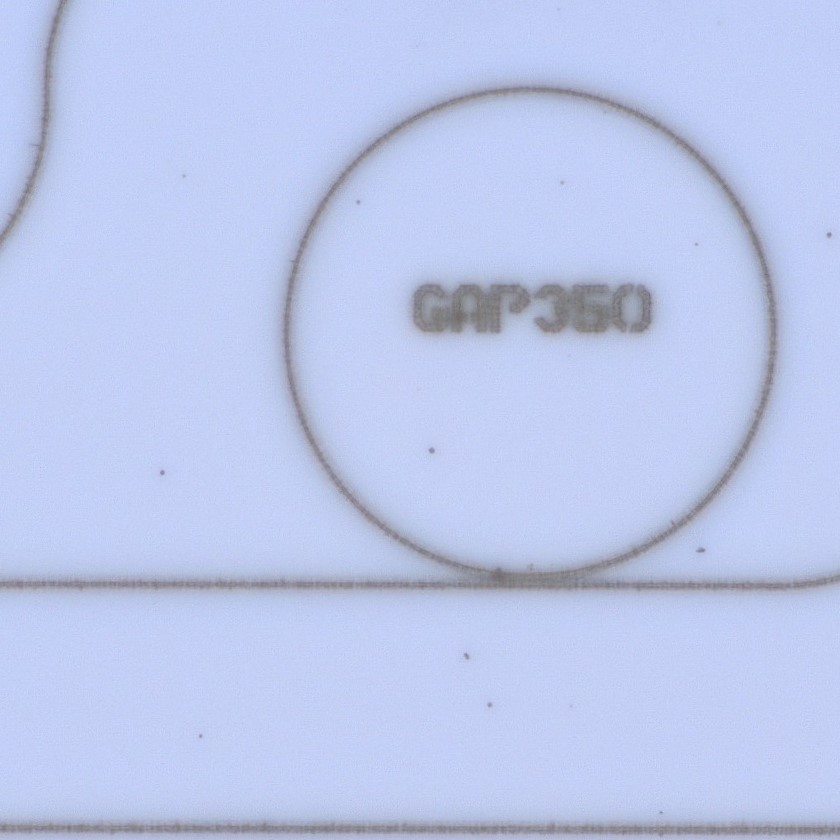
\includegraphics[width=\textwidth]{imgs/jpg/LS_ac}
    \caption{}
    \end{subfigure}
    \begin{subfigure}[b]{0.45\textwidth}
    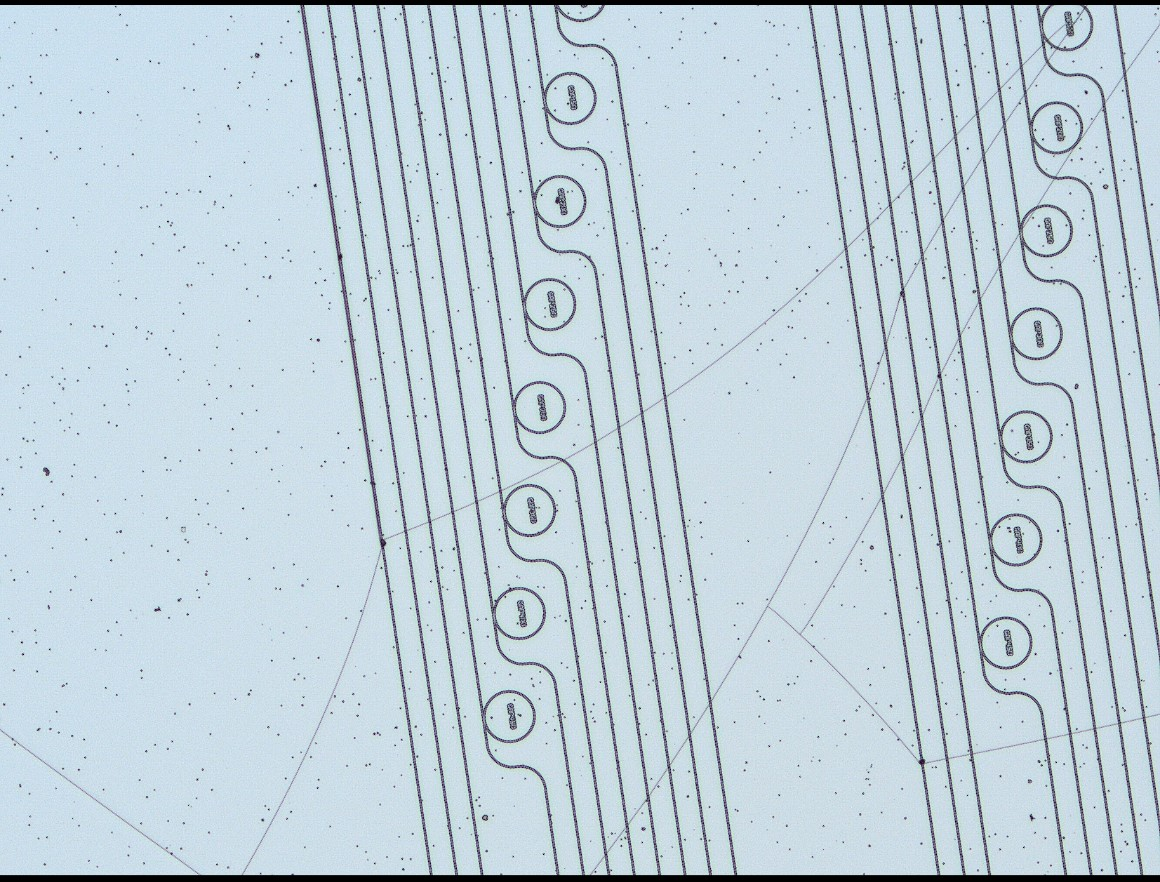
\includegraphics[width=\textwidth]{imgs/jpg/LS_tc}
    \caption{}
    \end{subfigure}    
    \begin{subfigure}[b]{0.45\textwidth}
    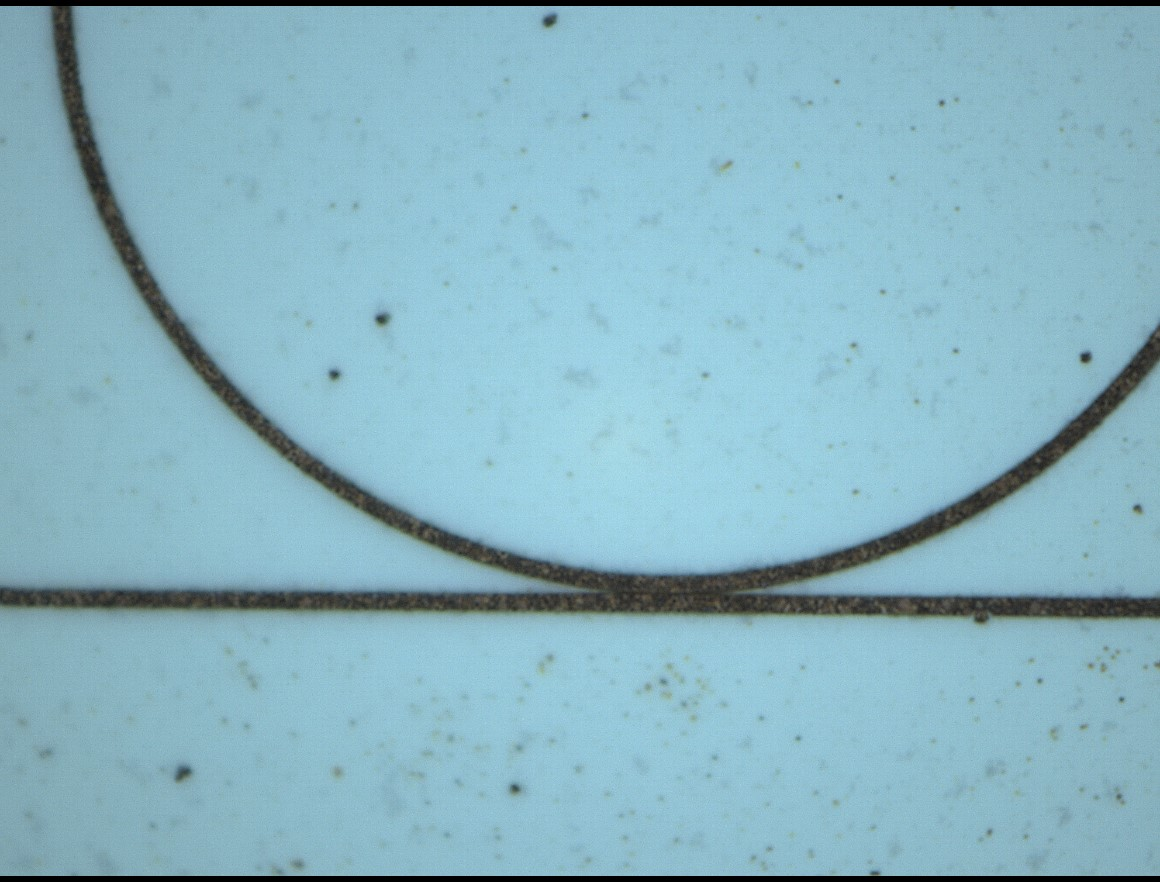
\includegraphics[width=\textwidth]{imgs/jpg/SR_ac}
    \caption{}
    \end{subfigure}
    \begin{subfigure}[b]{0.45\textwidth}
    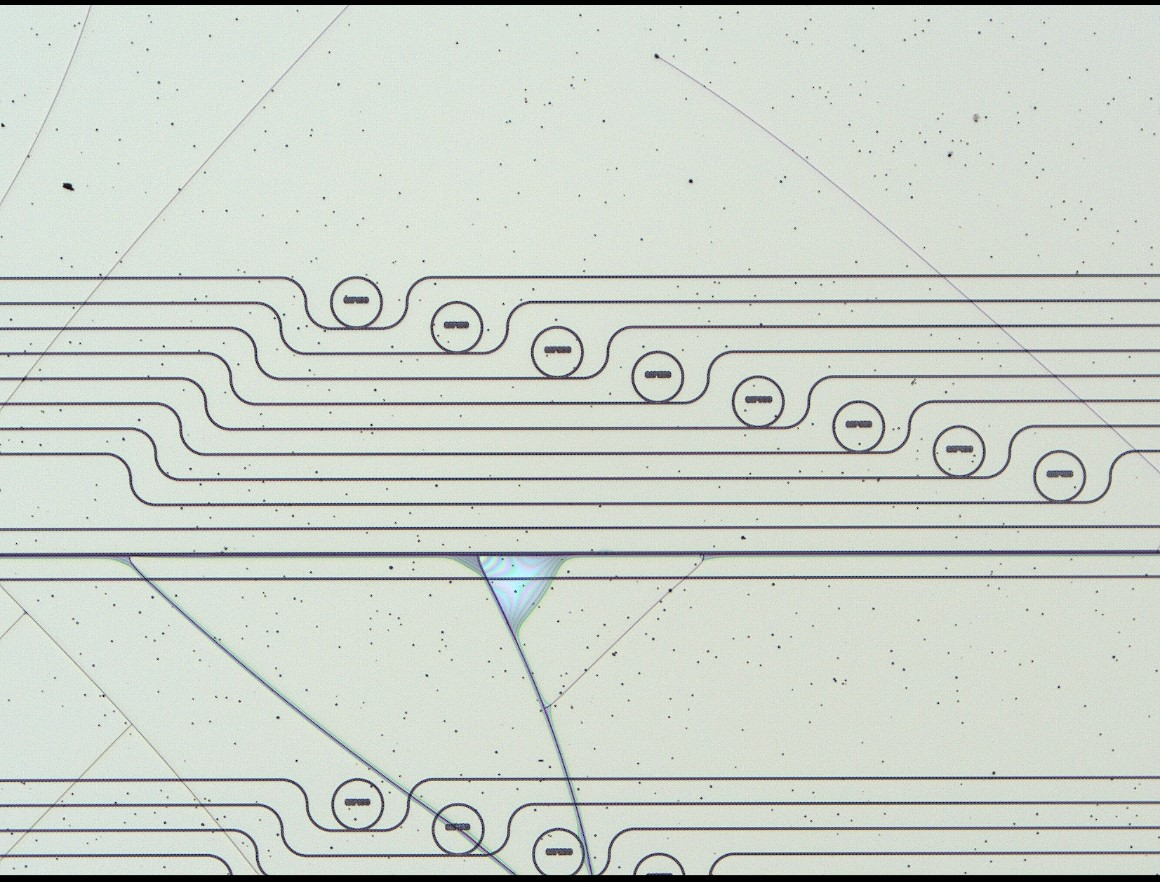
\includegraphics[width=\textwidth]{imgs/jpg/SR_tc}
    \caption{}
    \end{subfigure}
    \mycaption{Laser microscope images of samples after annealing process}{All the sample are annealed under the same circumstance. \textbf{a}. LS-CVD sample without top cladding. \textbf{b}. LS-CVD sample with TEOS top-cladding. \textbf{c}. PE-CVD sampele without top cladding. \textbf{d}. PE-CVD sample with TEOS top-cladding.}
    \label{fig:anneal}
\end{figure}

\subsection{Edge coupling and chip dicing}

In previous works \cite{Sunada2018}, both grating coupling and edge coupling were designed and studied. In this research, considering the broadband frequency conversion motivation, the edge coupling is preferred due to the broader 3 dB bandwidth. 

To achieve high coupling efficiency, we adopt monolithic inversed tapered waveguide as the mode convertor. The input and output ports of waveguide are both tapered from normal width 1.5 \si{\um} to a narrower end. By FDTD methods, the mode field is swept with different taper end widths.

\begin{figure}
	\centering
	\begin{subfigure}[b]{0.33\textwidth}
		\includesvg[width=\textwidth]{taper/03.svg}
		\caption{End width 0.3 \si{\um}}
	\end{subfigure}\hfill
	\begin{subfigure}[b]{0.33\textwidth}
		\includesvg[width=\textwidth]{taper/06}
		\caption{End width 0.6 \si{\um}}
	\end{subfigure}\hfill
	\begin{subfigure}[b]{0.33\textwidth}
		\includesvg[width=\textwidth]{taper/09}
		\caption{End width 0.9 \si{\um}}
	\end{subfigure}
	\vfill
	\begin{subfigure}[b]{0.33\textwidth}
		\includesvg[width=\textwidth]{taper/12}
		\caption{End width 1.2 \si{\um}}
	\end{subfigure}
	\begin{subfigure}[b]{0.33\textwidth}
		\includesvg[width=\textwidth]{taper/15}
		\caption{End width 1.5 \si{\um}}
	\end{subfigure}
    \mycaption{Mode field at the taper end}{The outline of taper edge is profiled.}
\label{fig:taper}
\end{figure}

From the result shown in \autoref{fig:taper}a, the mode fields expand horizontally as the taper end width increases proportionally. The largest mode size of 3.4 \si{\um} $\times$ 3.4 \si{\um} is successfully demonstrated, but the enhancement is not significant compared with no tapered port in \autoref{fig:taper}e. In result, a lensed fiber with spot diameter from 3.0 \si{\um} to 3.4 \si{\um} is recommended. 

In order to precisely define the input and output ports, the chip dicing is required.
Compared with conventional mechanical dicing,  the laser dicing technique is advantageous at high precision and less damages on the chip edges. The image of laser diced edge is compared with the manually diced one in \autoref{fig:dicing}. Apparently, the chip using laser dicing has smoother edge, which is helpful to reduce the backward scattering.

\begin{figure}
    \centering
	\begin{subfigure}[b]{0.45\textwidth}
		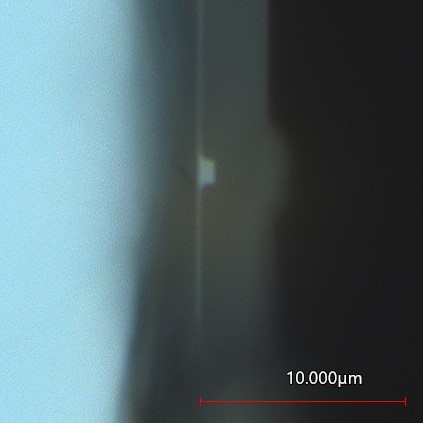
\includegraphics[width=\textwidth]{imgs/jpg/laser}
% 		\caption{Laser diced}
	\end{subfigure}
	\begin{subfigure}[b]{0.45\textwidth}
		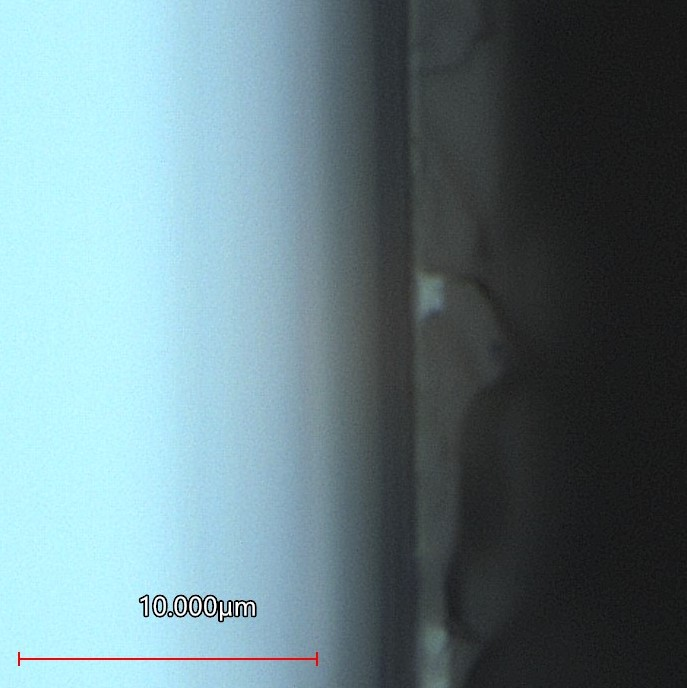
\includegraphics[width=\textwidth]{imgs/jpg/manual_cleav}
% 		\caption{Manually cleaved}
	\end{subfigure}
    \mycaption{Caption}{}
    \label{fig:dicing}
\end{figure}

\section{Fabless samples via foundries}

Fabless photonic research is becoming a trend for its cheaper and easier external run \cite{Hochberg2010}. There are several foundries all around the world offering the multi-project run service on integrated photonics and quantum optics applications, such as AMF in Singapore, Ligentec in Switterland, LioniX in Netherlands and etc. 

Based on the silicon nitride platform, two independent foundries are evaluated in the following sections in the term of device performance and fabrication techniques.

\subsection{Ligentec technique}
Photonic damascene process \cite{Pfeiffer2015a,Pfeiffer2018a} used in Ligentec samples improves the waveguide sidewall roughness by depositing the silicon nitride film into the etched thermal oxidized silica. By additive chemical mechanical planarization (CMP), the top surface of silicon nitride is also flatten.  

The laser microscope images is shown in . Several layers of different structures are found hierarchically, including the cross pattern stopping the crack during annealing and CMP, the silicon waveguides and a top unknown metallic layer.

\subsection{NTT-AT technique}

NTT-AT technique adopts a different physical vapor method--reactive sputtering to deposit non-hydrogen silicon nitride. Compared with standard silicon sputtering, the nitrogen flow is supplied and reacts with silicon vapor into the silicon nitride film. 

% Despite the hydrogen bond induced loss.
% !TeX root = ../main.tex

\chapter{Device evaluation and dispersion analysis}% from transmission spectroscopy

%\section{Methods}

In the example given in \autoref{sec:disp-comp},  a typical dispersive ring resonator has the $ D_2 $ value less than MHz, which means the frequency FSR, for example 100 GHz, is different from the next one with a MHz-level difference. It is difficult to achieve such precise measurement using traditional optical spectrum analyzer whose typical resolution is around pm, 100 MHz. The tunable laser scanning is developed to solve this problem, especially assisted by an external frequency comb \cite{Liu2016d}. 

Here, we exploit the method using laser step triggering to calibrate the real-time measured device transmission. Compared with the frequency comb or wave meter assisted spectroscopy, this method is much more convenient to deploy. By increasing the data acquisition sampling rate or altering with electric oscilloscope, the wavelength precision can be further improved.
Given the well-resonant spectrum, the dispersion information is further extracted from the transmission, in particular the resonant peaks. Such method is widely used to study the Kerr frequency comb. It is also efficient to study the frequency-entangled photon pair generation.

\section{Methods}

\subsection{Fiber launching}
Much of related works, concerning such as photonic crystals or whispering gallery mode resonators, use prism coupling or tapered fiber coupling for coupling tunability. 
%interact the external optical filed with cavity evanescent filed though, 
In the case of integrated ring resonators, the bus wavegudies are designed in the distance of several gaps, usually varying from under-coupling to over-coupling. 
Thus, the light confined in the bus waveguide can be directly coupled inwards or outwards using appropriate optical fibers. 
In previous works \cite{Sunada2018}, both grating coupling and edge coupling were adopted. However, considering the broadband frequency conversion motivation, the edge coupling is preferred for a comparatively broader 3-dB bandwidth. 
 
Using two five-axis fiber alignment stages (Newport M-562F-XYZ \& M-562F-XYZ-LH), the device ports are aligned with the lensed fiber on both sides. The spot size of lensed fibers is 2 \si{\um}, which is not optimized to the size mentioned in \autoref{sec:chip-dicing}.
In the case of ligentec samples,  the best facet-to-facet coupling efficiency is around 6 dB. 
Comparatively, a more typical facet-to-facet loss without mode convertors can be 8-9 dB.

%LS-CVD samples

It is worth mentioning that a chip arrier (SURUGA SEIKI F126) equipped with a thermoelectric cooler (TEC) is specialized for the \textit{xz}-axis device stage, which is essential for long-time thermal stability. 
With connected to an external temperature controller, the temperature precision of device under test can be .1 \si{\celsius}.
To prevent moisture condensation, the TEC is set a little bit higher than room temperature, 30 \si{\celsius} in our case. 

\subsection{Spectrum sweeping}

\begin{figure}
	\centering
	\includesvg[width=.9\textwidth]{trans_setup}
%	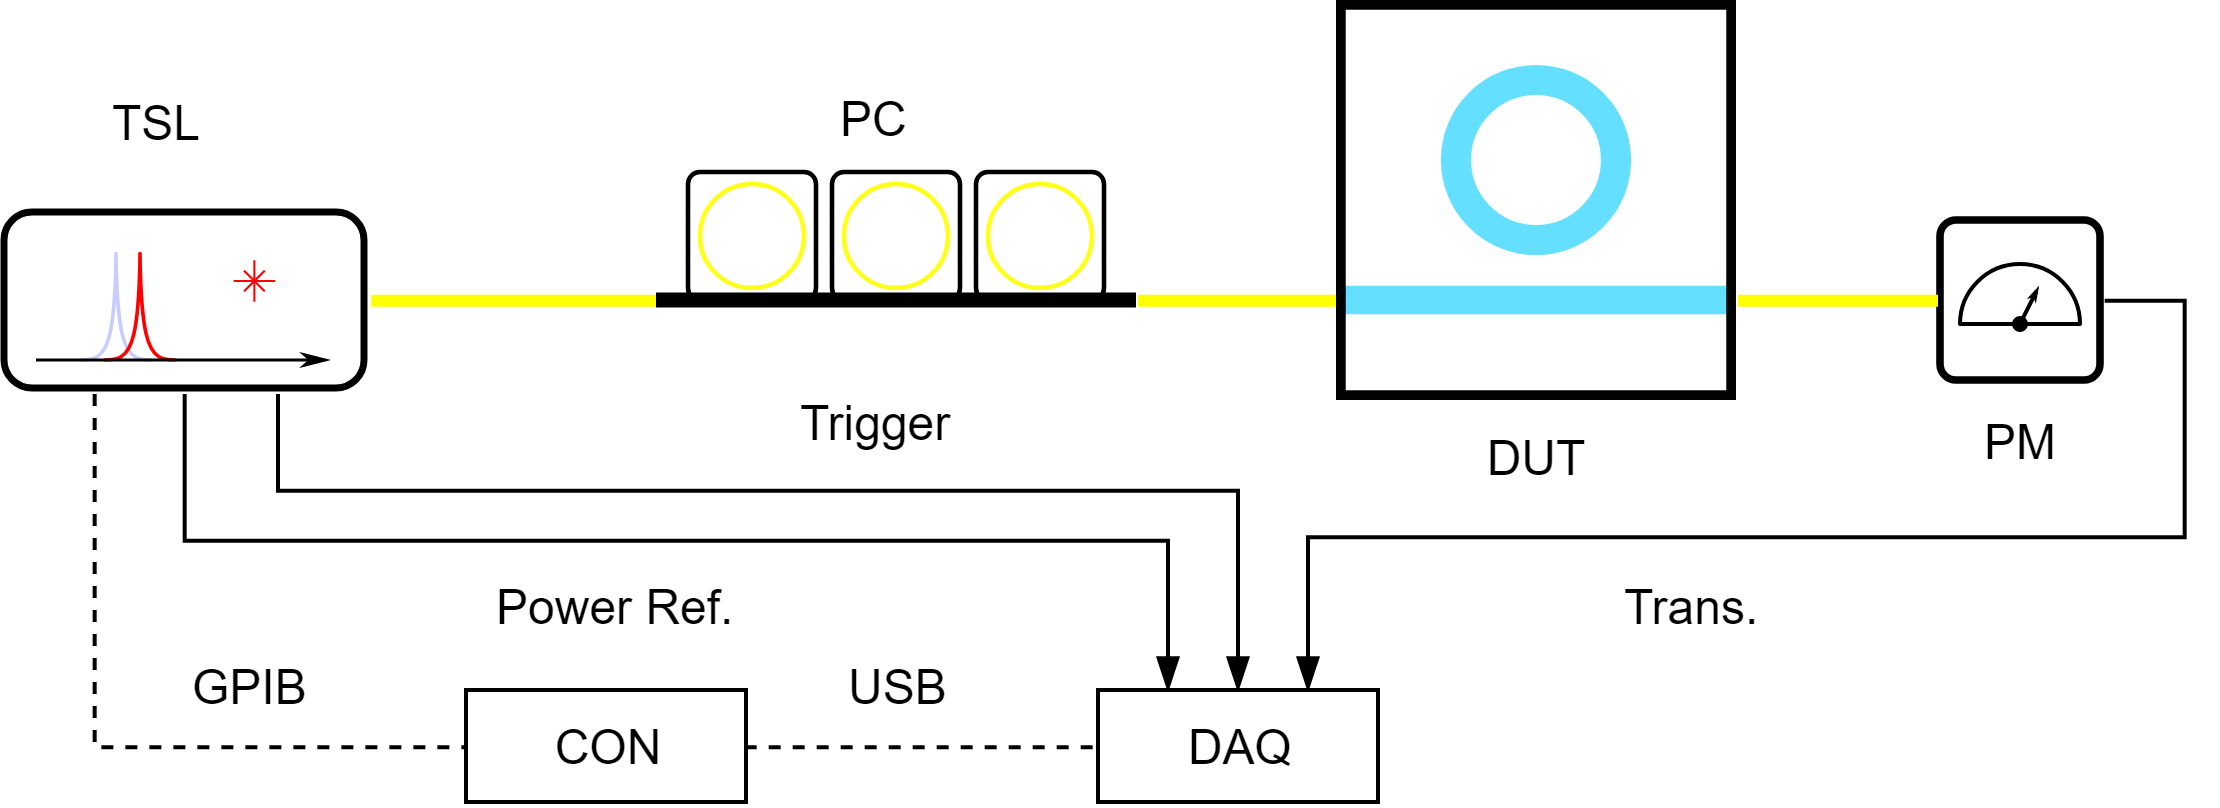
\includegraphics[width=.9\textwidth]{imgs/png/trans_setup}
	\mycaption{Setup of transmission measurement system}{TSL, tunable semiconductor laser. PC, optical fiber polarization controller. DUT, device under test. PM, power meter. DAQ, data acquisition.}
	\label{fig:transsetup}
\end{figure}

The schematic diagram of the device spectrum measurement is shown in \autoref{fig:transsetup}. Before the spectrum scanning, the output port is coupled to the infrared InGaAs camera in free space using a 20$\times$ objective lens. By carefully rotating the palette of polarization controller on the input side, the device can be launched in either TE or TM mode. Next, the TSL (SANTEC TSL-710) is set to continuously sweep from 1480 nm - 1640 nm, covering the telecom S C and L bands. The internal power reference signal and the step trigger are also generated simultaneously. Compared with photon diodes, the power meter (Newport 2963-R) in our setup is critical to realize the scanning at various power ranges.  Finally, the signals from power monitor, step trigger and device transmission are all synchronized with the data acquisition module, and then analyzed by the computer.

Given the transmission spectra, the negative peaks are located with peak-finding algorithm, yielding not only the peak location, but also the width and prominence, which are used to calculate the free spectral range and \textit{Q}-factor.

\section{Results}

\subsection{Thermal stability}

\begin{figure}
	\centering
	\includesvg[width=1\textwidth]{thermal}
	%	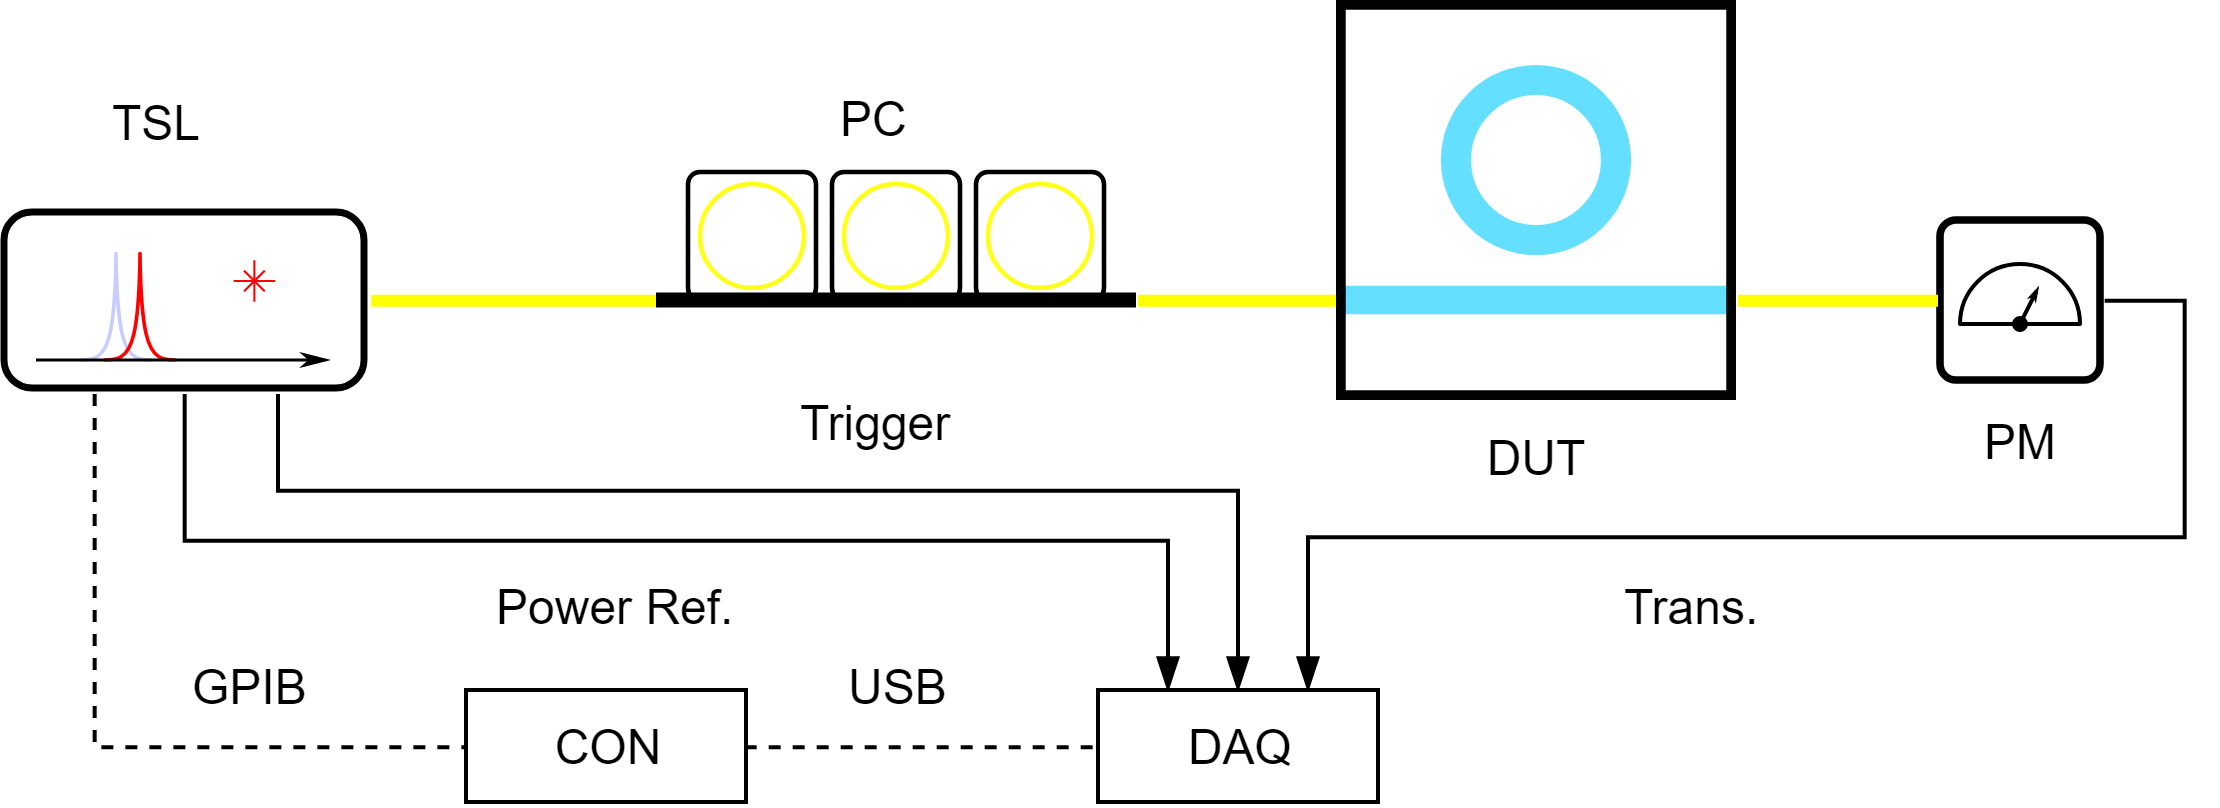
\includegraphics[width=.9\textwidth]{imgs/png/trans_setup}
	\mycaption{}{}
	\label{fig:thermal}
\end{figure}

%\begin{figure}
%	\centering
%	\includesvg[width=.9\textwidth]{dwldT}
%	%	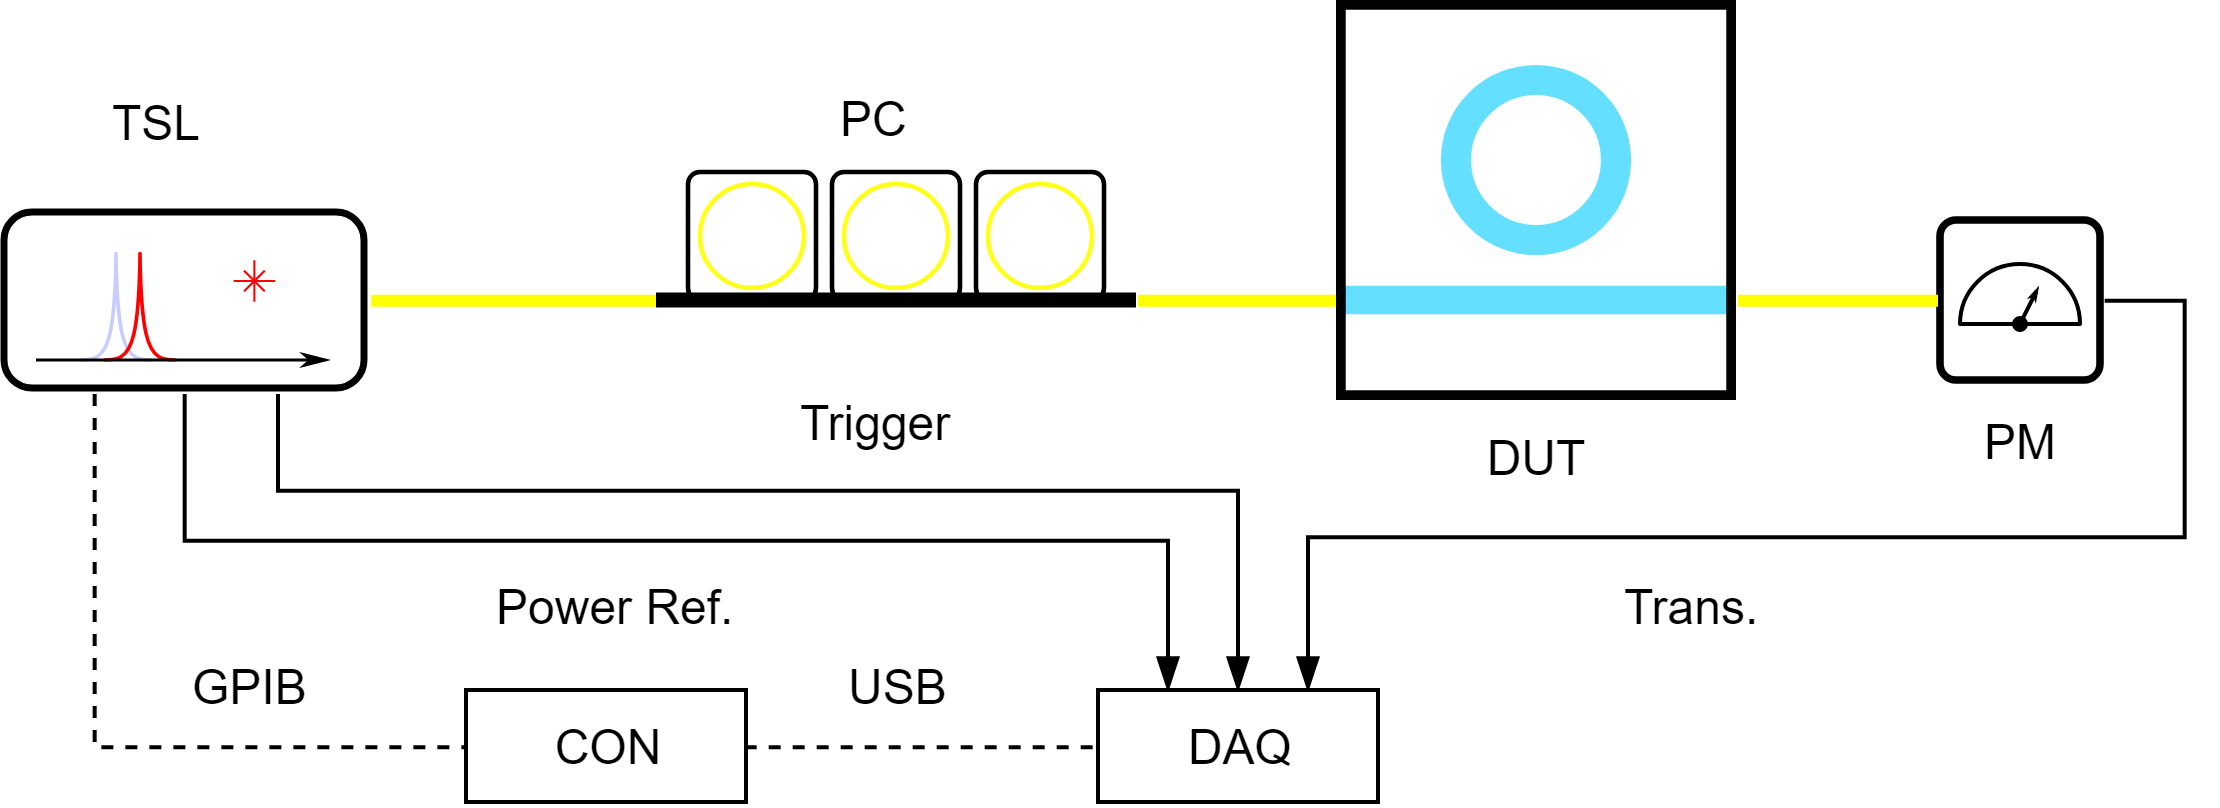
\includegraphics[width=.9\textwidth]{imgs/png/trans_setup}
%	\mycaption{}{}
%	\label{fig:wl-T}
%\end{figure}

Although silicon nitride is reported as high thermal conductivity material, the surrounding silicon dioxide is comparatively worse thermal-conductive. Despite the room temperature fluctuation, the nonlinear phenomena usually requires high pump power, which heats the device significantly, the index change variation leads to resonance shift. Thus, the thermal sensitivity is a critical factor of nonlinear ring resonators.

For example, with the TEC set into different temperatures, the spectrum of a LP-CVD sample is then measured. Shown in \autoref{fig:thermal}a, temperature increasing leads to a obvious red-shift of the resonant peak. The wavelength range around 1630 nm is chosen for better transmission and well resonance in this device. From \autoref{fig:thermal}b, the estimated thermal dependence of resonant wavelength $\dv*{\lambda}{T}$ is 23 \si{\nm/\celsius}. In this case, if the \textit{Q}-factor of ring resonator is up to \num{10d5}, even room temperature variation can results in resonance totally mismatching at pumping wavelength.

%\subsection{Device transmission}

\subsection{Substractive fabricated samples}

To compare the material difference among the films deposited in three CVD methods, identical layout is used to fabricate the ring resonators using all the same recipes. %Controlling thickness 
Since the thickness control during the film deposition and ICP etching are tough, all the device are label with the waveguide height measured by step profiler before TEOS top cladding.

The device transmission spectrum is first measured shown in \autoref{fig:trans_cf}. It can be seen that there is strong optical absorption from 1520 nm to 1540 nm in each device. Compared with the FTIR result shown in \autoref{fig:ftir}, in particular the case of LP-CVD sample where is almost no Si-H or N-H bonds found, the absorption at optical telecom band not only originates from the residual hydrogen but also may results in top-cladding or bottom buried TEOS layer.

 The radius of these device are fixed to 200 \si{\um}.

 transmission spectrum are compared. In 

\begin{figure}
	\centering
	\includesvg[width=.6\textwidth]{trans_cf}
	\mycaption{}{}
	\label{fig:trans_cf}
\end{figure}



\subsection{Dispersion analysis}

% !TeX root = ../main.tex

\chapter{Fabless samples via foundries}\label{chap:6}

Fabless photonic research is becoming a trend for its cheaper and easier external run \cite{Hochberg2010}. There are several foundries all around the world offering the multi-project run service on integrated photonics and quantum optics applications, such as AMF in Singapore, LIGENTEC in Switterland, LioniX in Netherlands and etc. 

Except standard subtractive process used in previous chapter, to discover fabrication process diversity, we also design the device layout and order the devices fablessly.
In the case of silicon nitride, two independent foundries are compared in the term of fabrication technique and device performance in the following sections.

\section{Fabless process}
The fabless sample involved in this research is ordered from LIGENTEC in Switzerland, and NTT-AT in Japan. Next, the process technique used is roughly introduced.

\bigskip
\noindent\textbf{LIGENTEC technique}

Photonic damascene process \cite{Pfeiffer2015a,Pfeiffer2018a} used in LIGENTEC samples improves the waveguide sidewall roughness by depositing the silicon nitride film into the etched thermal oxidized silica. By additive chemical mechanical planarization (CMP), the top surface of silicon nitride is polished.

The sample layout is illustrated in \autoref{fig:gds}. Five device groups with various FSRs are contained. In each specific group, the coupling gap is tuned from 400 nm to 700 nm in the step of 100 nm.

\begin{table}[]
	\mycaption{Design parameters of LIGENTEC samples}{FSR is specialized at 1550 nm.}
	\label{tab:ligentec}
	\begin{tabular}{cccc}
		% \hline
		& Ring Radius (\um) & FSR (GHz) & Ring Width (\um) \\ \hline
		Group 1 & 237.28                                                 & 100       & 0.8                                                   \\ \hline
		Group 2 & 157.95                                                 & 150       & 1.7                                                   \\ \hline
		Group 3 & 119.90                                                 & 200       & 1.5                                                   \\ \hline
		Group 4 & 78.55                                                  & 300       & 1.7                                                   \\ \hline
		Group 5 & 22.95                                                  & 1000      & 1.7                                                   \\ \hline
	\end{tabular}
\end{table}

The microscope images of the sample is shown in \autoref{fig:LIGENTEC-laser-micro}. Several layers of different structures are observed hierarchically, including the cross pattern stopping the crack during annealing and CMP, the waveguide layer and a top metallic layer for other users in the same run.

\begin{figure}
	\centering
	\includesvg[width=5in]{gds}
	\mycaption{Layout of fabless samples}{\textbf{a} is the layout of NTT-AT sample, including the identical design of LIGENTEC device shown in \textbf{b}. The cell size is 1mm$\times$1mm. }
	\label{fig:gds}
\end{figure}

\begin{figure}
	\centering
	\includesvg[width=4in]{ligentec/ligentec_image}
	\mycaption{Laser microscope images of LIGENTEC samples}{By lowering the focus depth, three layers are observed.
		\textbf{a}. Top metallic layer. \textbf{b}. Device layer. \textbf{c}. Crack stopper layer. \textbf{d}. Mode convertor. The metallic bar is 30\um-long.}
	\label{fig:LIGENTEC-laser-micro}
\end{figure}

\bigskip
\noindent\textbf{NTT-AT technique}

NTT-AT technique adopts a different physical vapor method--reactive sputtering to deposit non-hydrogen silicon nitride. Compared with standard silicon sputtering, silicon atoms emitted from source react with the nitrogen gas flow into silicon nitride. Refractive index of the film deposited using this method is included in \autoref{fig:ellipso}.

In the term of design, the 4-inch wafer is customized with 22 cell in the layout shown in \autoref{fig:gds}, including the same design of LIGENTEC one in the special cell.

\section{Device evaluation}

\subsection{Coupling evolution}

Prior to cavity property evaluation, it is essential to compare the coupling condition among devices in the same group. Since the gap between bus waveguide and ring resonator is swept increasingly, usually the coupling condition turns from over coupling to critical coupling, and finally into weak coupling.

For the LIGENTEC Group 1, due to the reliable fabrication process, such an evolution of coupling condition is explicit. Presented in \autoref{fig:gap_cf}(a), the coupling condition varies from over coupling to critical coupling, as the negative prominence of resonance peak increases. This tendency agrees with the \textit{Q}-factor counts, shown in \autoref{fig:gap_cf}(b). The other groups in the sample have similar feature but the critical coupling gaps are different.

\begin{figure}
	\centering
	\includesvg[width=5in]{ligentec/gap_cf}
	\mycaption{Transmission and \textit{Q}-factors of devices sweeping the gap}{The coupling condition varies from over coupling to critical coupling, as the negative prominence of resonance peak increases in \textbf{a}. The same tendency agrees with the \textit{Q}-factors in \textbf{b}.}
	\label{fig:gap_cf}
\end{figure}

%\subsection{Deterministic dispersion compensation}

\subsection{Dispersion inversion}

Thanks to the high quality fabrication of LIGENTEC damascene process, Group 1 and Group 2 show interesting dispersion inversion as ring widths increase. Presented in \autoref{fig:dint_comp}, as the ring width is tuned from 0.8 \um to 1.7 \um, the mode dispersion is inversed significantly, from -0.83 MHz to 1.46 MHz.

\begin{figure}
	\centering
	\includesvg[width=4.5in]{fabless/dint_comp}
	\mycaption{Dispersion inversion shown by integrated dispersion}{The ring width is tuned from 0.8 \um (Group 1) to 1.7 \um (Group 2), the mode dispersion is inversed significantly.}
	\label{fig:dint_comp}
\end{figure}


\subsection{Comparison of quality factor and dispersion}


Several works using the same LIGENTEC technique report ultrahigh \textit{Q}-factors up to \num{3d6} \cites{Yu2019, Vaidya2019}. The same magnitude is also attained in our samples in Group 3 and Group 5. While to compare the fabrication quality of both technique, two device with the same design (Group 1 Device 4, gap 700nm, FSR 100 GHz, ring width 0.8 \um ) are listed in \autoref{fig:fabless_cf}, as well as the \textit{Q}-factor histograms.

\begin{figure}
	\centering
	\includesvg[width=4in]{fabless/fabless_cf}
	\mycaption{A comparison between identical ring resonator fabricated using LIGENTEC and NTT-AT technique}{\textbf{a}. Transmission, \textit{Q}-factors, FSR of LIGENTC sample. \textbf{b}. Transmission, \textit{Q}-factors, FSR of NTT-AT sample. \textit{Q}-factors histogram of LIGENTEC and NTT-AT are given in \textbf{c} and \textbf{d} respectively. Identical pattern is used for fabrication (Group 1 Device 4, gap 700nm, FSR 100 GHz, ring width 0.8 \um). }
	\label{fig:fabless_cf}
\end{figure}

In the transmission of LIGENTEC device, shown in \autoref{fig:fabless_cf}(a)  and NTT-AT device shown in \autoref{fig:fabless_cf}(b), there is no obvious absorption in the range 1500 nm - 1540 nm compared with the samples fabricated using non-annealing subtractive recipe
%, though the transmission background declines at both red and blue side. 
However, the quality factors of LIGENTEC ones are almost 4 times higher than NTT-AT.
%, indicating the intracavity loss is 4 times lower. 
The histogram gathered in \autoref{fig:fabless_cf}(c) and \autoref{fig:fabless_cf}(b) features the same result.
In both samples, the critical coupling features at shorter wavelength, according to the peak prominence and \textit{Q}-factor tendency. 

We assume that despite the ammonia-free recipe used in NTT-AT technique, the etching recipe is not as fully optimized as LIGENTEC ones. It is also interesting to find that there is a clear difference of FSR trends from the former. In particular, the increasing NTT-AT FSRs indicate a normal dispersion.

%\subsection{Dispersion comparison}

The identical devices mentioned above is further analyzed using the above method. The integrated dispersion is extracted in \autoref{fig:dint_cf}. As we can see, the fabrication process influence the dispersion effectively as a result of different film growing technology is performed.

\begin{figure}
	\centering
	\includesvg[width=4.5in]{fabless/dint_cf}
	\mycaption{Comparison of integrated dispersion between LIGENTEC and NTT-AT samples with same device parameters}{Fabrication process changes the dispersion effectively as a result of different film growing technology is performed.}
	\label{fig:dint_cf}
\end{figure}
% !TeX root = ../main.tex
\chapter{Broadband photon pair generation}

Back to the classical nonlinear optics theory, the solution to nonlinear coupling equations requires the initial power at ether signal or idler mode, which is called seed in the laser terminology. However, in quantum optics theory, all the modes in cavity behave intrinsic vacuum fluctuation at the quantity of half $ \hbar \omega $. Thus, even without light fed, the quantum fluctuation leads to emission at the single photon levels. 

Furthermore, intracavity pump power then behaves the amplifier, intensify the corresponding signal or idler mode photon flux. Once the single photon flux exceeds cavity threshold, the extracavity single photon can be detected. To note, these kind of excitation is indistinguishable because the signal and idler photons are emitted simultaneously as a result of quantum mechanics, rather than signal photon stimulates idler photon and vice versa. In the context of quantum states, the state created intracavity is at the superposition of signal state and idler state. The wave packet is different from the normal single photon one. Further theoretical research \cite{Scully1997} explained the squeezed nature of four wave mixing photon pairs, which is one of the exclusive properties of frequency entangled photon pairs.

In general, the spontaneous four wave mixing in nonlinear cavities defined in our context refers to the cavity modes are excited collectively and pair-by-pair under the phase matching condition. Thus, under the weak coherent approximation, the photon pair only include one photon in each mode but correlated with each other. Thus, the conventional coincidence counting technology can be used to verify such correlation. In the term of generation band, it agrees with the classical phase matching condition at pump power limit.

%Furthermore, 
%To clarify with the physics compared with the relevant research, such as Kerr frequency comb and soliton generation, where ultra-high power is used to built intracavity pump mode, the spontaneous four wave mixing differs 
%\cite{Chembo2016a}

\section{Methods}

Using the dispersion extraction method in previous chapter, zero dispersion wavelength can be located easily among the measured band. In our experiments, optical telecom band, especially C band is focused on, because enormous fiber optical components, like in-line filters are available in this range.

Illustrated in \autoref{fig:bibpf}, the setup of mode-resolvable singular photon pair generation first adopts the tunable laser as pump source, whose display tunability is 0.1 pm and able to be tuned via external voltage input. The laser output is connected to ring resonators using the fiber launching system and the output power is measured with the power meter. 

A simple transmission scanning is then perform to select the built-in polarization.
For the high \textit{Q}-factor devices, the transmission of TE and TM modes are separated in a distance of tens of pm. Thus, as either of the resonance vanished by rotating the polarization controller, the fiber launches the particular polarization mode of bus waveguide. For low \textit{Q}-factor cavities, since the TE and TM are degenerate in the spectrum, the method of polarization alignment is as same as the one using the InGaAs infrared camera.

Beyond the polarization selection, the pump wavelength should also be aligned to the resonance of ring resonators. The on-resonance or off-resonance can be determined as the output displays largest distinction ratio. In our experiment, the pump peak around 1550 nm, usually perform at least 10 dB extinction ratio between on-resonance and off-resonance.

Next, the output light are splitted 50\si{\percent} by 50\si{\percent} into signal and idler channels, indicating half of generated photons are lost. The two channels are sequentially filtered through two sets of band pass filters. The 3dB bandwidth in the first set is 1540$\pm$4 nm and 1560$\pm$4 nm, respectively. The second set of band pass filters are 0.01nm-tunable and 3dB bandwith is 0.12nm. Since mode spacing, FSR in our device is much more larger, the tunable band pass filter is adequate to pass only single mode.

Finally, each channel are detected by superconducting single photon detectors (SNSPD) which are specific for infrared range. The time resolution is 100 ps. Since the SNSPD is polarization-sensitive, another two polarization controllers (not shown) are used to achieve maximal single photon counting during each measurement. At last, the time controller (ID Quantique, ID900) collects and records the counting time tag in the 100 ps resolution. The coincidence counting is triggered directly or calculated by setting the coincidence window. 

\begin{figure}
	\centering
	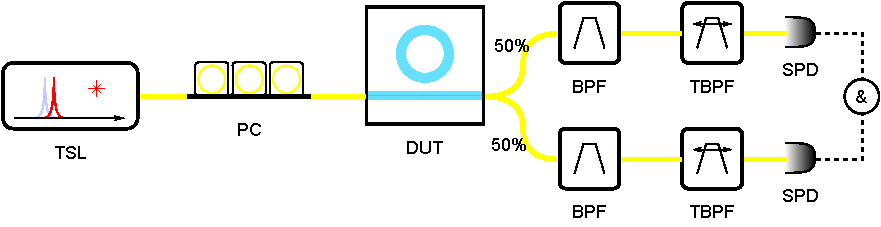
\includegraphics[width=1\linewidth]{imgs/biBPF.pdf}
%	\includesvg[width=.9\textwidth]{setup/biBPF}
	\mycaption{Mode-resolvable singular photon pair generation}{}
	\label{fig:bibpf}
\end{figure}

\bigskip
\textbf{Coincidence counting}

In quantum optics, coincidence counting is usually used to examine the non-locality of singular wave-particle. In our case, the photons which are splitted into two channels A and B yields the count per second $N_\mathrm{A}$ and $ N_\mathrm{B} $. Define the coincidence windows $t$, 1 ns commonly, and coincidence count (CC) is two photon trigger events within this small time window, equivalent to the photon pair generation rate effectively. The accidental counting (ACC) is defined as $ N_\mathrm{A} N_\mathrm{B} t $, similar to the background noise of counting system. Thus accidental-coincidence ratio (CAR) is defined as (CC-ACC)/ACC to reduce the noise effects.

It is worth to mention that in our research, the main topic is photon pair generation rather than photn state manipulation, in result numerous band-pass filters are exploited to realize mode-resolvable single photon counting. It does not contradict with distinguishability nature of frequency correlated photon pairs.


\section{Low power photon pair generation}

\subsection{Single mode photon flux}

With the pump power set as 100 \si{\micro\watt} and central wavelength at 1550.64 nm, the result of photon flux of both signal and idler bands versus relative mode index is presented in \autoref{fig:flux1}. The device deployed has FSR of 150 GHz and shows anomalous dispersion around 1550 nm. According to the 3dB bandwidth of band pass filters, the accessible relative mode index corresponds 7-14. To achieve higher photon counting, the central wavelength of TBPFs is tuned carefully in the step of 0.01 nm.

In the result, there is trend that both signal and idler photon fluxes decreases as the mode index increases. It can be explained that phase mismatch of farther modes is greater than closer ones. The difference between signal and idler bands origins from the asymmetry of phase matching condition and filter spectral shape. As the input power is set as 100 \si{\micro\watt}, the estimated photon generation rate is around \num{d3} per mode per \si{\micro\watt}.

\begin{figure}
	\centering
	\includesvg[width=5in]{mode_depen/flux_1}
	\mycaption{Photon flux at 100 \si{\micro\watt} of Ligentec group 2 device 1}{The pump power set as 100 \si{\micro\watt} and central pump wavelength is at 1550.64 nm. Selected modes is from 1536 nm to 1544 nm for idler band and 1556 nm to 1564 nm for signal band.}
	\label{fig:flux1}
\end{figure}


\subsection{Coincidence counts of singular mode pair}

In coincidence counts are measured in a 1ns coincidence window and in each mode, the time delay is set from -200 to 200 ps. The \autoref{fig:mode_cf} shows the result of coincidence counts and CAR. In the mode pair 9, single photo pair generation rate is 1500 per second, equals to \num{1.5d4} per mW, which is the highest rate observed at this input power level among all the samples.

As the mode number increases, coincidence counts varies roughly but in the CAR graph, such a trend is not obvious. This is due to the band pass filters used in our setup is not flat-top on the transmission spectrum. In conclusion, even several frequency-dependent optical components used in our setup, by calculating the coincidence-accidental ratio, the photon pair generation behavior can be analyzed precisely.

\begin{figure}
	\centering
	\includesvg[width=6in]{mode_depen/mode_cf}
	\mycaption{Photon flux at 100 \si{\micro\watt} of Ligentec group 2 device 1}{}
	\label{fig:mode_cf}
\end{figure}

\section{Pump power dependence}

Since the spontaneous four wave mixing originates from Kerr nonlinearity, in classical nonlinear optics, converted power is linearly dependent on pump power. To confirm this relation in quantum scale, it is necessary to study both power dependence of photon flux and coincidence counts.

To amplify the pump power, a erbium-doped fiber amplifier (EDFA) is cascaded after the tunable laser. By increasing the output power, the power intracavity can exceed 500 mW. 
The mode passed through is fixed at $ \mu=9 $ ,corresponding to $\lambda_\mathrm{i}$ = 1540.28 nm and $\lambda_\mathrm{s}$ = 1558.79 nm. During each peak resonance alignment, the extinction ratio is around 10 dB. 
The result of photo flux is given in \autoref{fig:pwflux}. It is apparent that there is a continual growth of photon flux in both signal and idler modes. 

\begin{figure}
	\centering
	\includesvg[width=3in]{pw_depen/pw_flux}
	\mycaption{}{}
	\label{fig:pwflux}
\end{figure}

\begin{figure}
	\centering
	\includesvg[width=6in]{pw_depen/pw_cc_acc}
	\mycaption{}{}
	\label{fig:pwcar}
\end{figure}

Furthermore, the coincidence counting result is shown in \autoref{fig:pwcar}(a) where both maximal coincidence counts and background accidental coincidence counts increase with the pump power. While from CAR provided in \autoref{fig:pwcar}(b), higher input power leads to a significant decline. This can explained by the background noise arising from the Raman effect in optical fibers \cite{Engin2012}
. As the nonlinearity of optical fiber is much weaker than silicon nitride device, in the high input power regime, it becomes obvious and contributes to the single photo count while decreasing the coincidence count rate.

\section{Joint spectrum intensity}

Since the spontaneous four wave mixing occurs simultaneously at each mode pair, the state generated in a broadband is equivalent to the intensity superposition all over the signal and idler bands. To clarify the quantum state characteristics in this view, usually the joint spectrum filed or intensity is measured to evaluate the frequency correlation \cites{Helt2010,Vernon2015b}. For example, compared with the $ N $ mode correlation measurement mentioned above, the joint spectrum intensity requires the coincidence measurement over the whole two-party $ N^2 $ hibert space.

\subsection{Setups}

Much of recent research concerning soliton generation discussed the thermal stability in the nonlinear ring resonators \cites{Guo2017a,Herr2012}. 

To solve this problem, illustrated in \autoref{fig:pid}, an auxiliary photon detector is added to monitor off-resonance. Using digital proportional–integral–derivative (PID) controller, which is realize by a LabVIEW program, the wavelength of tunable laser is tuned dynamically by the external voltage input. In this way, the extinction ratio of our system can keep at a low level as soon as possible. In addition, to increase the available mode number, the first set of band pass filter in \autoref{fig:bibpf} is replaced by a notch filter. 

\begin{figure}
	\centering
	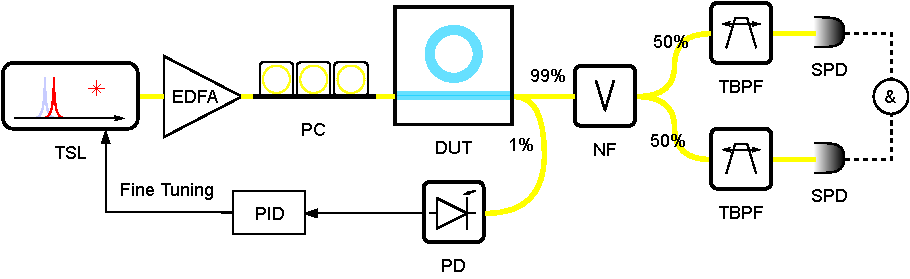
\includegraphics[width=1\linewidth]{imgs/pid.pdf}
	%	\includesvg[width=.9\textwidth]{setup/biBPF}
	\caption{}
	\label{fig:pid}
\end{figure}

\autoref{fig:jsi} presents the final results of intermodal coincidence counts, accidental coincidence counts and their ratio, CAR. The operation 

\begin{figure}
	\centering
	\includesvg[width=5in]{jsi/flux_2}
	\mycaption{Photon flux at 100 \si{\micro\watt} of Ligentec group 2 device 1}{}
	\label{fig:flux2}
\end{figure}

\begin{figure}
	\centering
	\includesvg[width=6in]{jsi/jsi_map}
	\mycaption{}{}
	\label{fig:jsi}
\end{figure}






\begin{acknowledgements}
\lipsum[2-4]
\end{acknowledgements}

% \bibliography{library}
% \bibliographystyle{kueethesis}
% \bibliographystyle{unsrt}
\printbibliography[title=References,heading=bibintoc]

\clearpage % ensure all floats are processed
\processdelayedfloats
\clearpage

\begin{appendices}
\chapter{Dispersion simulation}
\chapter{Layout design}
\end{appendices}

\end{document}
